% Generated by generate_nine_templates.py from the archived order-23 instances.
\begin{figure}[!htbp]
\centering
\begin{tabular}{@{}c@{\hspace{2.5mm}}c@{\hspace{2.5mm}}c@{\hspace{2.5mm}}c@{}}
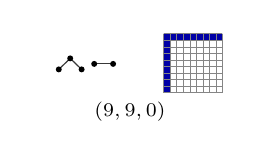
\begin{tikzpicture}[x=1mm,y=1mm,baseline=0mm]
\path[use as bounding box] (0,-1) rectangle (27,11);
\draw[black!78,line width=.43pt] (5.40,7.10)--(3.95,5.70) (5.40,7.10)--(6.85,5.70);
\fill (5.40,7.10) circle[radius=.38mm];
\fill (3.95,5.70) circle[radius=.38mm];
\fill (6.85,5.70) circle[radius=.38mm];
\draw[black!78,line width=.43pt] (8.45,6.40)--(10.85,6.40);
\fill (8.45,6.40) circle[radius=.38mm];
\fill (10.85,6.40) circle[radius=.38mm];
\begin{scope}[shift={(17.265,2.765)},x=0.83mm,y=0.83mm]
\fill[blue!65!black] (0,0) rectangle (1,9) (0,8) rectangle (9,9);
\draw[black!48,line width=.16pt] (0,0)--(0,9) (1,0)--(1,9) (2,0)--(2,9) (3,0)--(3,9) (4,0)--(4,9) (5,0)--(5,9) (6,0)--(6,9) (7,0)--(7,9) (8,0)--(8,9) (9,0)--(9,9) (0,0)--(9,0) (0,1)--(9,1) (0,2)--(9,2) (0,3)--(9,3) (0,4)--(9,4) (0,5)--(9,5) (0,6)--(9,6) (0,7)--(9,7) (0,8)--(9,8) (0,9)--(9,9);
\end{scope}
\node[font=\scriptsize,inner sep=0pt] at (13,.35) {$(9,9,0)$};
\end{tikzpicture} &
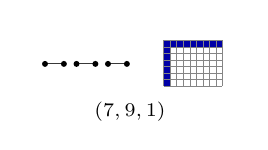
\begin{tikzpicture}[x=1mm,y=1mm,baseline=0mm]
\path[use as bounding box] (0,-1) rectangle (27,11);
\draw[black!78,line width=.43pt] (2.20,6.40)--(4.60,6.40);
\fill (2.20,6.40) circle[radius=.38mm];
\fill (4.60,6.40) circle[radius=.38mm];
\draw[black!78,line width=.43pt] (6.20,6.40)--(8.60,6.40);
\fill (6.20,6.40) circle[radius=.38mm];
\fill (8.60,6.40) circle[radius=.38mm];
\draw[black!78,line width=.43pt] (10.20,6.40)--(12.60,6.40);
\fill (10.20,6.40) circle[radius=.38mm];
\fill (12.60,6.40) circle[radius=.38mm];
\begin{scope}[shift={(17.265,3.595)},x=0.83mm,y=0.83mm]
\fill[blue!65!black] (0,0) rectangle (1,7) (0,6) rectangle (9,7);
\draw[black!48,line width=.16pt] (0,0)--(0,7) (1,0)--(1,7) (2,0)--(2,7) (3,0)--(3,7) (4,0)--(4,7) (5,0)--(5,7) (6,0)--(6,7) (7,0)--(7,7) (8,0)--(8,7) (9,0)--(9,7) (0,0)--(9,0) (0,1)--(9,1) (0,2)--(9,2) (0,3)--(9,3) (0,4)--(9,4) (0,5)--(9,5) (0,6)--(9,6) (0,7)--(9,7);
\end{scope}
\node[font=\scriptsize,inner sep=0pt] at (13,.35) {$(7,9,1)$};
\end{tikzpicture} &
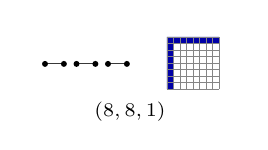
\begin{tikzpicture}[x=1mm,y=1mm,baseline=0mm]
\path[use as bounding box] (0,-1) rectangle (27,11);
\draw[black!78,line width=.43pt] (2.20,6.40)--(4.60,6.40);
\fill (2.20,6.40) circle[radius=.38mm];
\fill (4.60,6.40) circle[radius=.38mm];
\draw[black!78,line width=.43pt] (6.20,6.40)--(8.60,6.40);
\fill (6.20,6.40) circle[radius=.38mm];
\fill (8.60,6.40) circle[radius=.38mm];
\draw[black!78,line width=.43pt] (10.20,6.40)--(12.60,6.40);
\fill (10.20,6.40) circle[radius=.38mm];
\fill (12.60,6.40) circle[radius=.38mm];
\begin{scope}[shift={(17.680,3.180)},x=0.83mm,y=0.83mm]
\fill[blue!65!black] (0,0) rectangle (1,8) (0,7) rectangle (8,8);
\draw[black!48,line width=.16pt] (0,0)--(0,8) (1,0)--(1,8) (2,0)--(2,8) (3,0)--(3,8) (4,0)--(4,8) (5,0)--(5,8) (6,0)--(6,8) (7,0)--(7,8) (8,0)--(8,8) (0,0)--(8,0) (0,1)--(8,1) (0,2)--(8,2) (0,3)--(8,3) (0,4)--(8,4) (0,5)--(8,5) (0,6)--(8,6) (0,7)--(8,7) (0,8)--(8,8);
\end{scope}
\node[font=\scriptsize,inner sep=0pt] at (13,.35) {$(8,8,1)$};
\end{tikzpicture} &
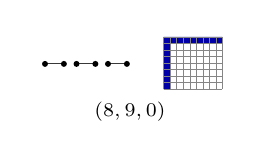
\begin{tikzpicture}[x=1mm,y=1mm,baseline=0mm]
\path[use as bounding box] (0,-1) rectangle (27,11);
\draw[black!78,line width=.43pt] (2.20,6.40)--(4.60,6.40);
\fill (2.20,6.40) circle[radius=.38mm];
\fill (4.60,6.40) circle[radius=.38mm];
\draw[black!78,line width=.43pt] (6.20,6.40)--(8.60,6.40);
\fill (6.20,6.40) circle[radius=.38mm];
\fill (8.60,6.40) circle[radius=.38mm];
\draw[black!78,line width=.43pt] (10.20,6.40)--(12.60,6.40);
\fill (10.20,6.40) circle[radius=.38mm];
\fill (12.60,6.40) circle[radius=.38mm];
\begin{scope}[shift={(17.265,3.180)},x=0.83mm,y=0.83mm]
\fill[blue!65!black] (0,0) rectangle (1,8) (0,7) rectangle (9,8);
\draw[black!48,line width=.16pt] (0,0)--(0,8) (1,0)--(1,8) (2,0)--(2,8) (3,0)--(3,8) (4,0)--(4,8) (5,0)--(5,8) (6,0)--(6,8) (7,0)--(7,8) (8,0)--(8,8) (9,0)--(9,8) (0,0)--(9,0) (0,1)--(9,1) (0,2)--(9,2) (0,3)--(9,3) (0,4)--(9,4) (0,5)--(9,5) (0,6)--(9,6) (0,7)--(9,7) (0,8)--(9,8);
\end{scope}
\node[font=\scriptsize,inner sep=0pt] at (13,.35) {$(8,9,0)$};
\end{tikzpicture} \\[.5mm]
\end{tabular}
\caption{Order-23 templates with 3 unmarked edges. Each panel gives the unmarked graph, the chain matrix and $(a,c,i)$.}
\label{fig:nine-chain-1}
\end{figure}

\begin{figure}[!htbp]
\centering
\begin{tabular}{@{}c@{\hspace{2.5mm}}c@{\hspace{2.5mm}}c@{\hspace{2.5mm}}c@{}}
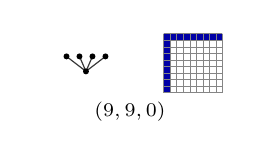
\begin{tikzpicture}[x=1mm,y=1mm,baseline=0mm]
\path[use as bounding box] (0,-1) rectangle (27,11);
\draw[black!78,line width=.43pt] (7.40,5.45)--(4.93,7.35) (7.40,5.45)--(6.58,7.35) (7.40,5.45)--(8.23,7.35) (7.40,5.45)--(9.88,7.35);
\fill (7.40,5.45) circle[radius=.38mm];
\fill (4.93,7.35) circle[radius=.38mm];
\fill (6.58,7.35) circle[radius=.38mm];
\fill (8.23,7.35) circle[radius=.38mm];
\fill (9.88,7.35) circle[radius=.38mm];
\begin{scope}[shift={(17.265,2.765)},x=0.83mm,y=0.83mm]
\fill[blue!65!black] (0,0) rectangle (1,9) (0,8) rectangle (9,9);
\draw[black!48,line width=.16pt] (0,0)--(0,9) (1,0)--(1,9) (2,0)--(2,9) (3,0)--(3,9) (4,0)--(4,9) (5,0)--(5,9) (6,0)--(6,9) (7,0)--(7,9) (8,0)--(8,9) (9,0)--(9,9) (0,0)--(9,0) (0,1)--(9,1) (0,2)--(9,2) (0,3)--(9,3) (0,4)--(9,4) (0,5)--(9,5) (0,6)--(9,6) (0,7)--(9,7) (0,8)--(9,8) (0,9)--(9,9);
\end{scope}
\node[font=\scriptsize,inner sep=0pt] at (13,.35) {$(9,9,0)$};
\end{tikzpicture} &
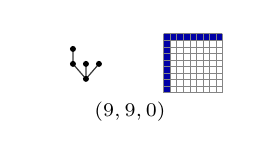
\begin{tikzpicture}[x=1mm,y=1mm,baseline=0mm]
\path[use as bounding box] (0,-1) rectangle (27,11);
\draw[black!78,line width=.43pt] (7.40,4.50)--(5.75,6.40) (7.40,4.50)--(7.40,6.40) (7.40,4.50)--(9.05,6.40) (5.75,6.40)--(5.75,8.30);
\fill (7.40,4.50) circle[radius=.38mm];
\fill (5.75,6.40) circle[radius=.38mm];
\fill (7.40,6.40) circle[radius=.38mm];
\fill (9.05,6.40) circle[radius=.38mm];
\fill (5.75,8.30) circle[radius=.38mm];
\begin{scope}[shift={(17.265,2.765)},x=0.83mm,y=0.83mm]
\fill[blue!65!black] (0,0) rectangle (1,9) (0,8) rectangle (9,9);
\draw[black!48,line width=.16pt] (0,0)--(0,9) (1,0)--(1,9) (2,0)--(2,9) (3,0)--(3,9) (4,0)--(4,9) (5,0)--(5,9) (6,0)--(6,9) (7,0)--(7,9) (8,0)--(8,9) (9,0)--(9,9) (0,0)--(9,0) (0,1)--(9,1) (0,2)--(9,2) (0,3)--(9,3) (0,4)--(9,4) (0,5)--(9,5) (0,6)--(9,6) (0,7)--(9,7) (0,8)--(9,8) (0,9)--(9,9);
\end{scope}
\node[font=\scriptsize,inner sep=0pt] at (13,.35) {$(9,9,0)$};
\end{tikzpicture} &
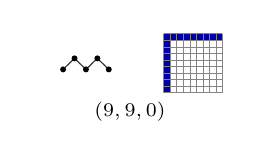
\begin{tikzpicture}[x=1mm,y=1mm,baseline=0mm]
\path[use as bounding box] (0,-1) rectangle (27,11);
\draw[black!78,line width=.43pt] (7.40,5.70)--(5.95,7.10) (7.40,5.70)--(8.85,7.10) (5.95,7.10)--(4.50,5.70) (8.85,7.10)--(10.30,5.70);
\fill (7.40,5.70) circle[radius=.38mm];
\fill (5.95,7.10) circle[radius=.38mm];
\fill (8.85,7.10) circle[radius=.38mm];
\fill (4.50,5.70) circle[radius=.38mm];
\fill (10.30,5.70) circle[radius=.38mm];
\begin{scope}[shift={(17.265,2.765)},x=0.83mm,y=0.83mm]
\fill[blue!65!black] (0,0) rectangle (1,9) (0,8) rectangle (9,9);
\draw[black!48,line width=.16pt] (0,0)--(0,9) (1,0)--(1,9) (2,0)--(2,9) (3,0)--(3,9) (4,0)--(4,9) (5,0)--(5,9) (6,0)--(6,9) (7,0)--(7,9) (8,0)--(8,9) (9,0)--(9,9) (0,0)--(9,0) (0,1)--(9,1) (0,2)--(9,2) (0,3)--(9,3) (0,4)--(9,4) (0,5)--(9,5) (0,6)--(9,6) (0,7)--(9,7) (0,8)--(9,8) (0,9)--(9,9);
\end{scope}
\node[font=\scriptsize,inner sep=0pt] at (13,.35) {$(9,9,0)$};
\end{tikzpicture} &
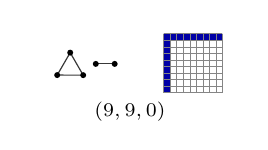
\begin{tikzpicture}[x=1mm,y=1mm,baseline=0mm]
\path[use as bounding box] (0,-1) rectangle (27,11);
\draw[black!78,line width=.43pt] (5.40,7.83)--(3.75,4.98) (5.40,7.83)--(7.05,4.97) (3.75,4.98)--(7.05,4.97);
\fill (5.40,7.83) circle[radius=.38mm];
\fill (3.75,4.98) circle[radius=.38mm];
\fill (7.05,4.97) circle[radius=.38mm];
\draw[black!78,line width=.43pt] (8.65,6.40)--(11.05,6.40);
\fill (8.65,6.40) circle[radius=.38mm];
\fill (11.05,6.40) circle[radius=.38mm];
\begin{scope}[shift={(17.265,2.765)},x=0.83mm,y=0.83mm]
\fill[blue!65!black] (0,0) rectangle (1,9) (0,8) rectangle (9,9);
\draw[black!48,line width=.16pt] (0,0)--(0,9) (1,0)--(1,9) (2,0)--(2,9) (3,0)--(3,9) (4,0)--(4,9) (5,0)--(5,9) (6,0)--(6,9) (7,0)--(7,9) (8,0)--(8,9) (9,0)--(9,9) (0,0)--(9,0) (0,1)--(9,1) (0,2)--(9,2) (0,3)--(9,3) (0,4)--(9,4) (0,5)--(9,5) (0,6)--(9,6) (0,7)--(9,7) (0,8)--(9,8) (0,9)--(9,9);
\end{scope}
\node[font=\scriptsize,inner sep=0pt] at (13,.35) {$(9,9,0)$};
\end{tikzpicture} \\[.5mm]
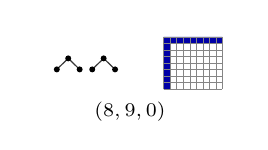
\begin{tikzpicture}[x=1mm,y=1mm,baseline=0mm]
\path[use as bounding box] (0,-1) rectangle (27,11);
\draw[black!78,line width=.43pt] (5.15,7.10)--(3.70,5.70) (5.15,7.10)--(6.60,5.70);
\fill (5.15,7.10) circle[radius=.38mm];
\fill (3.70,5.70) circle[radius=.38mm];
\fill (6.60,5.70) circle[radius=.38mm];
\draw[black!78,line width=.43pt] (9.65,7.10)--(8.20,5.70) (9.65,7.10)--(11.10,5.70);
\fill (9.65,7.10) circle[radius=.38mm];
\fill (8.20,5.70) circle[radius=.38mm];
\fill (11.10,5.70) circle[radius=.38mm];
\begin{scope}[shift={(17.265,3.180)},x=0.83mm,y=0.83mm]
\fill[blue!65!black] (0,0) rectangle (1,8) (0,7) rectangle (9,8);
\draw[black!48,line width=.16pt] (0,0)--(0,8) (1,0)--(1,8) (2,0)--(2,8) (3,0)--(3,8) (4,0)--(4,8) (5,0)--(5,8) (6,0)--(6,8) (7,0)--(7,8) (8,0)--(8,8) (9,0)--(9,8) (0,0)--(9,0) (0,1)--(9,1) (0,2)--(9,2) (0,3)--(9,3) (0,4)--(9,4) (0,5)--(9,5) (0,6)--(9,6) (0,7)--(9,7) (0,8)--(9,8);
\end{scope}
\node[font=\scriptsize,inner sep=0pt] at (13,.35) {$(8,9,0)$};
\end{tikzpicture} &
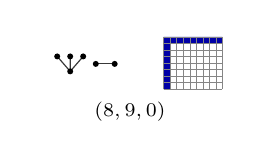
\begin{tikzpicture}[x=1mm,y=1mm,baseline=0mm]
\path[use as bounding box] (0,-1) rectangle (27,11);
\draw[black!78,line width=.43pt] (5.40,5.45)--(3.75,7.35) (5.40,5.45)--(5.40,7.35) (5.40,5.45)--(7.05,7.35);
\fill (5.40,5.45) circle[radius=.38mm];
\fill (3.75,7.35) circle[radius=.38mm];
\fill (5.40,7.35) circle[radius=.38mm];
\fill (7.05,7.35) circle[radius=.38mm];
\draw[black!78,line width=.43pt] (8.65,6.40)--(11.05,6.40);
\fill (8.65,6.40) circle[radius=.38mm];
\fill (11.05,6.40) circle[radius=.38mm];
\begin{scope}[shift={(17.265,3.180)},x=0.83mm,y=0.83mm]
\fill[blue!65!black] (0,0) rectangle (1,8) (0,7) rectangle (9,8);
\draw[black!48,line width=.16pt] (0,0)--(0,8) (1,0)--(1,8) (2,0)--(2,8) (3,0)--(3,8) (4,0)--(4,8) (5,0)--(5,8) (6,0)--(6,8) (7,0)--(7,8) (8,0)--(8,8) (9,0)--(9,8) (0,0)--(9,0) (0,1)--(9,1) (0,2)--(9,2) (0,3)--(9,3) (0,4)--(9,4) (0,5)--(9,5) (0,6)--(9,6) (0,7)--(9,7) (0,8)--(9,8);
\end{scope}
\node[font=\scriptsize,inner sep=0pt] at (13,.35) {$(8,9,0)$};
\end{tikzpicture} &
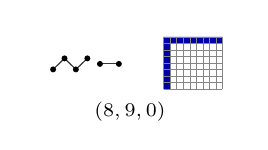
\begin{tikzpicture}[x=1mm,y=1mm,baseline=0mm]
\path[use as bounding box] (0,-1) rectangle (27,11);
\draw[black!78,line width=.43pt] (4.68,7.10)--(6.12,5.70) (4.68,7.10)--(3.23,5.70) (6.12,5.70)--(7.58,7.10);
\fill (4.68,7.10) circle[radius=.38mm];
\fill (6.12,5.70) circle[radius=.38mm];
\fill (3.23,5.70) circle[radius=.38mm];
\fill (7.58,7.10) circle[radius=.38mm];
\draw[black!78,line width=.43pt] (9.18,6.40)--(11.58,6.40);
\fill (9.18,6.40) circle[radius=.38mm];
\fill (11.58,6.40) circle[radius=.38mm];
\begin{scope}[shift={(17.265,3.180)},x=0.83mm,y=0.83mm]
\fill[blue!65!black] (0,0) rectangle (1,8) (0,7) rectangle (9,8);
\draw[black!48,line width=.16pt] (0,0)--(0,8) (1,0)--(1,8) (2,0)--(2,8) (3,0)--(3,8) (4,0)--(4,8) (5,0)--(5,8) (6,0)--(6,8) (7,0)--(7,8) (8,0)--(8,8) (9,0)--(9,8) (0,0)--(9,0) (0,1)--(9,1) (0,2)--(9,2) (0,3)--(9,3) (0,4)--(9,4) (0,5)--(9,5) (0,6)--(9,6) (0,7)--(9,7) (0,8)--(9,8);
\end{scope}
\node[font=\scriptsize,inner sep=0pt] at (13,.35) {$(8,9,0)$};
\end{tikzpicture} &
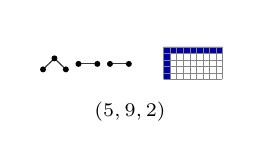
\begin{tikzpicture}[x=1mm,y=1mm,baseline=0mm]
\path[use as bounding box] (0,-1) rectangle (27,11);
\draw[black!78,line width=.43pt] (3.40,7.10)--(1.95,5.70) (3.40,7.10)--(4.85,5.70);
\fill (3.40,7.10) circle[radius=.38mm];
\fill (1.95,5.70) circle[radius=.38mm];
\fill (4.85,5.70) circle[radius=.38mm];
\draw[black!78,line width=.43pt] (6.45,6.40)--(8.85,6.40);
\fill (6.45,6.40) circle[radius=.38mm];
\fill (8.85,6.40) circle[radius=.38mm];
\draw[black!78,line width=.43pt] (10.45,6.40)--(12.85,6.40);
\fill (10.45,6.40) circle[radius=.38mm];
\fill (12.85,6.40) circle[radius=.38mm];
\begin{scope}[shift={(17.265,4.425)},x=0.83mm,y=0.83mm]
\fill[blue!65!black] (0,0) rectangle (1,5) (0,4) rectangle (9,5);
\draw[black!48,line width=.16pt] (0,0)--(0,5) (1,0)--(1,5) (2,0)--(2,5) (3,0)--(3,5) (4,0)--(4,5) (5,0)--(5,5) (6,0)--(6,5) (7,0)--(7,5) (8,0)--(8,5) (9,0)--(9,5) (0,0)--(9,0) (0,1)--(9,1) (0,2)--(9,2) (0,3)--(9,3) (0,4)--(9,4) (0,5)--(9,5);
\end{scope}
\node[font=\scriptsize,inner sep=0pt] at (13,.35) {$(5,9,2)$};
\end{tikzpicture} \\[.5mm]
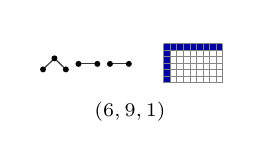
\begin{tikzpicture}[x=1mm,y=1mm,baseline=0mm]
\path[use as bounding box] (0,-1) rectangle (27,11);
\draw[black!78,line width=.43pt] (3.40,7.10)--(1.95,5.70) (3.40,7.10)--(4.85,5.70);
\fill (3.40,7.10) circle[radius=.38mm];
\fill (1.95,5.70) circle[radius=.38mm];
\fill (4.85,5.70) circle[radius=.38mm];
\draw[black!78,line width=.43pt] (6.45,6.40)--(8.85,6.40);
\fill (6.45,6.40) circle[radius=.38mm];
\fill (8.85,6.40) circle[radius=.38mm];
\draw[black!78,line width=.43pt] (10.45,6.40)--(12.85,6.40);
\fill (10.45,6.40) circle[radius=.38mm];
\fill (12.85,6.40) circle[radius=.38mm];
\begin{scope}[shift={(17.265,4.010)},x=0.83mm,y=0.83mm]
\fill[blue!65!black] (0,0) rectangle (1,6) (0,5) rectangle (9,6);
\draw[black!48,line width=.16pt] (0,0)--(0,6) (1,0)--(1,6) (2,0)--(2,6) (3,0)--(3,6) (4,0)--(4,6) (5,0)--(5,6) (6,0)--(6,6) (7,0)--(7,6) (8,0)--(8,6) (9,0)--(9,6) (0,0)--(9,0) (0,1)--(9,1) (0,2)--(9,2) (0,3)--(9,3) (0,4)--(9,4) (0,5)--(9,5) (0,6)--(9,6);
\end{scope}
\node[font=\scriptsize,inner sep=0pt] at (13,.35) {$(6,9,1)$};
\end{tikzpicture} &
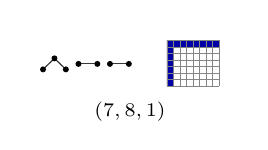
\begin{tikzpicture}[x=1mm,y=1mm,baseline=0mm]
\path[use as bounding box] (0,-1) rectangle (27,11);
\draw[black!78,line width=.43pt] (3.40,7.10)--(1.95,5.70) (3.40,7.10)--(4.85,5.70);
\fill (3.40,7.10) circle[radius=.38mm];
\fill (1.95,5.70) circle[radius=.38mm];
\fill (4.85,5.70) circle[radius=.38mm];
\draw[black!78,line width=.43pt] (6.45,6.40)--(8.85,6.40);
\fill (6.45,6.40) circle[radius=.38mm];
\fill (8.85,6.40) circle[radius=.38mm];
\draw[black!78,line width=.43pt] (10.45,6.40)--(12.85,6.40);
\fill (10.45,6.40) circle[radius=.38mm];
\fill (12.85,6.40) circle[radius=.38mm];
\begin{scope}[shift={(17.680,3.595)},x=0.83mm,y=0.83mm]
\fill[blue!65!black] (0,0) rectangle (1,7) (0,6) rectangle (8,7);
\draw[black!48,line width=.16pt] (0,0)--(0,7) (1,0)--(1,7) (2,0)--(2,7) (3,0)--(3,7) (4,0)--(4,7) (5,0)--(5,7) (6,0)--(6,7) (7,0)--(7,7) (8,0)--(8,7) (0,0)--(8,0) (0,1)--(8,1) (0,2)--(8,2) (0,3)--(8,3) (0,4)--(8,4) (0,5)--(8,5) (0,6)--(8,6) (0,7)--(8,7);
\end{scope}
\node[font=\scriptsize,inner sep=0pt] at (13,.35) {$(7,8,1)$};
\end{tikzpicture} &
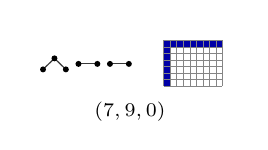
\begin{tikzpicture}[x=1mm,y=1mm,baseline=0mm]
\path[use as bounding box] (0,-1) rectangle (27,11);
\draw[black!78,line width=.43pt] (3.40,7.10)--(1.95,5.70) (3.40,7.10)--(4.85,5.70);
\fill (3.40,7.10) circle[radius=.38mm];
\fill (1.95,5.70) circle[radius=.38mm];
\fill (4.85,5.70) circle[radius=.38mm];
\draw[black!78,line width=.43pt] (6.45,6.40)--(8.85,6.40);
\fill (6.45,6.40) circle[radius=.38mm];
\fill (8.85,6.40) circle[radius=.38mm];
\draw[black!78,line width=.43pt] (10.45,6.40)--(12.85,6.40);
\fill (10.45,6.40) circle[radius=.38mm];
\fill (12.85,6.40) circle[radius=.38mm];
\begin{scope}[shift={(17.265,3.595)},x=0.83mm,y=0.83mm]
\fill[blue!65!black] (0,0) rectangle (1,7) (0,6) rectangle (9,7);
\draw[black!48,line width=.16pt] (0,0)--(0,7) (1,0)--(1,7) (2,0)--(2,7) (3,0)--(3,7) (4,0)--(4,7) (5,0)--(5,7) (6,0)--(6,7) (7,0)--(7,7) (8,0)--(8,7) (9,0)--(9,7) (0,0)--(9,0) (0,1)--(9,1) (0,2)--(9,2) (0,3)--(9,3) (0,4)--(9,4) (0,5)--(9,5) (0,6)--(9,6) (0,7)--(9,7);
\end{scope}
\node[font=\scriptsize,inner sep=0pt] at (13,.35) {$(7,9,0)$};
\end{tikzpicture} &
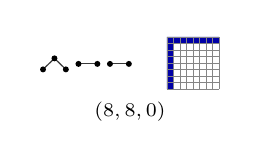
\begin{tikzpicture}[x=1mm,y=1mm,baseline=0mm]
\path[use as bounding box] (0,-1) rectangle (27,11);
\draw[black!78,line width=.43pt] (3.40,7.10)--(1.95,5.70) (3.40,7.10)--(4.85,5.70);
\fill (3.40,7.10) circle[radius=.38mm];
\fill (1.95,5.70) circle[radius=.38mm];
\fill (4.85,5.70) circle[radius=.38mm];
\draw[black!78,line width=.43pt] (6.45,6.40)--(8.85,6.40);
\fill (6.45,6.40) circle[radius=.38mm];
\fill (8.85,6.40) circle[radius=.38mm];
\draw[black!78,line width=.43pt] (10.45,6.40)--(12.85,6.40);
\fill (10.45,6.40) circle[radius=.38mm];
\fill (12.85,6.40) circle[radius=.38mm];
\begin{scope}[shift={(17.680,3.180)},x=0.83mm,y=0.83mm]
\fill[blue!65!black] (0,0) rectangle (1,8) (0,7) rectangle (8,8);
\draw[black!48,line width=.16pt] (0,0)--(0,8) (1,0)--(1,8) (2,0)--(2,8) (3,0)--(3,8) (4,0)--(4,8) (5,0)--(5,8) (6,0)--(6,8) (7,0)--(7,8) (8,0)--(8,8) (0,0)--(8,0) (0,1)--(8,1) (0,2)--(8,2) (0,3)--(8,3) (0,4)--(8,4) (0,5)--(8,5) (0,6)--(8,6) (0,7)--(8,7) (0,8)--(8,8);
\end{scope}
\node[font=\scriptsize,inner sep=0pt] at (13,.35) {$(8,8,0)$};
\end{tikzpicture} \\[.5mm]
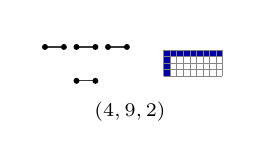
\begin{tikzpicture}[x=1mm,y=1mm,baseline=0mm]
\path[use as bounding box] (0,-1) rectangle (27,11);
\draw[black!78,line width=.43pt] (2.20,8.55)--(4.60,8.55);
\fill (2.20,8.55) circle[radius=.38mm];
\fill (4.60,8.55) circle[radius=.38mm];
\draw[black!78,line width=.43pt] (6.20,8.55)--(8.60,8.55);
\fill (6.20,8.55) circle[radius=.38mm];
\fill (8.60,8.55) circle[radius=.38mm];
\draw[black!78,line width=.43pt] (10.20,8.55)--(12.60,8.55);
\fill (10.20,8.55) circle[radius=.38mm];
\fill (12.60,8.55) circle[radius=.38mm];
\draw[black!78,line width=.43pt] (6.20,4.25)--(8.60,4.25);
\fill (6.20,4.25) circle[radius=.38mm];
\fill (8.60,4.25) circle[radius=.38mm];
\begin{scope}[shift={(17.265,4.840)},x=0.83mm,y=0.83mm]
\fill[blue!65!black] (0,0) rectangle (1,4) (0,3) rectangle (9,4);
\draw[black!48,line width=.16pt] (0,0)--(0,4) (1,0)--(1,4) (2,0)--(2,4) (3,0)--(3,4) (4,0)--(4,4) (5,0)--(5,4) (6,0)--(6,4) (7,0)--(7,4) (8,0)--(8,4) (9,0)--(9,4) (0,0)--(9,0) (0,1)--(9,1) (0,2)--(9,2) (0,3)--(9,3) (0,4)--(9,4);
\end{scope}
\node[font=\scriptsize,inner sep=0pt] at (13,.35) {$(4,9,2)$};
\end{tikzpicture} &
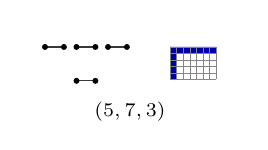
\begin{tikzpicture}[x=1mm,y=1mm,baseline=0mm]
\path[use as bounding box] (0,-1) rectangle (27,11);
\draw[black!78,line width=.43pt] (2.20,8.55)--(4.60,8.55);
\fill (2.20,8.55) circle[radius=.38mm];
\fill (4.60,8.55) circle[radius=.38mm];
\draw[black!78,line width=.43pt] (6.20,8.55)--(8.60,8.55);
\fill (6.20,8.55) circle[radius=.38mm];
\fill (8.60,8.55) circle[radius=.38mm];
\draw[black!78,line width=.43pt] (10.20,8.55)--(12.60,8.55);
\fill (10.20,8.55) circle[radius=.38mm];
\fill (12.60,8.55) circle[radius=.38mm];
\draw[black!78,line width=.43pt] (6.20,4.25)--(8.60,4.25);
\fill (6.20,4.25) circle[radius=.38mm];
\fill (8.60,4.25) circle[radius=.38mm];
\begin{scope}[shift={(18.095,4.425)},x=0.83mm,y=0.83mm]
\fill[blue!65!black] (0,0) rectangle (1,5) (0,4) rectangle (7,5);
\draw[black!48,line width=.16pt] (0,0)--(0,5) (1,0)--(1,5) (2,0)--(2,5) (3,0)--(3,5) (4,0)--(4,5) (5,0)--(5,5) (6,0)--(6,5) (7,0)--(7,5) (0,0)--(7,0) (0,1)--(7,1) (0,2)--(7,2) (0,3)--(7,3) (0,4)--(7,4) (0,5)--(7,5);
\end{scope}
\node[font=\scriptsize,inner sep=0pt] at (13,.35) {$(5,7,3)$};
\end{tikzpicture} &
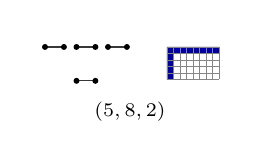
\begin{tikzpicture}[x=1mm,y=1mm,baseline=0mm]
\path[use as bounding box] (0,-1) rectangle (27,11);
\draw[black!78,line width=.43pt] (2.20,8.55)--(4.60,8.55);
\fill (2.20,8.55) circle[radius=.38mm];
\fill (4.60,8.55) circle[radius=.38mm];
\draw[black!78,line width=.43pt] (6.20,8.55)--(8.60,8.55);
\fill (6.20,8.55) circle[radius=.38mm];
\fill (8.60,8.55) circle[radius=.38mm];
\draw[black!78,line width=.43pt] (10.20,8.55)--(12.60,8.55);
\fill (10.20,8.55) circle[radius=.38mm];
\fill (12.60,8.55) circle[radius=.38mm];
\draw[black!78,line width=.43pt] (6.20,4.25)--(8.60,4.25);
\fill (6.20,4.25) circle[radius=.38mm];
\fill (8.60,4.25) circle[radius=.38mm];
\begin{scope}[shift={(17.680,4.425)},x=0.83mm,y=0.83mm]
\fill[blue!65!black] (0,0) rectangle (1,5) (0,4) rectangle (8,5);
\draw[black!48,line width=.16pt] (0,0)--(0,5) (1,0)--(1,5) (2,0)--(2,5) (3,0)--(3,5) (4,0)--(4,5) (5,0)--(5,5) (6,0)--(6,5) (7,0)--(7,5) (8,0)--(8,5) (0,0)--(8,0) (0,1)--(8,1) (0,2)--(8,2) (0,3)--(8,3) (0,4)--(8,4) (0,5)--(8,5);
\end{scope}
\node[font=\scriptsize,inner sep=0pt] at (13,.35) {$(5,8,2)$};
\end{tikzpicture} &
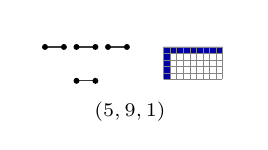
\begin{tikzpicture}[x=1mm,y=1mm,baseline=0mm]
\path[use as bounding box] (0,-1) rectangle (27,11);
\draw[black!78,line width=.43pt] (2.20,8.55)--(4.60,8.55);
\fill (2.20,8.55) circle[radius=.38mm];
\fill (4.60,8.55) circle[radius=.38mm];
\draw[black!78,line width=.43pt] (6.20,8.55)--(8.60,8.55);
\fill (6.20,8.55) circle[radius=.38mm];
\fill (8.60,8.55) circle[radius=.38mm];
\draw[black!78,line width=.43pt] (10.20,8.55)--(12.60,8.55);
\fill (10.20,8.55) circle[radius=.38mm];
\fill (12.60,8.55) circle[radius=.38mm];
\draw[black!78,line width=.43pt] (6.20,4.25)--(8.60,4.25);
\fill (6.20,4.25) circle[radius=.38mm];
\fill (8.60,4.25) circle[radius=.38mm];
\begin{scope}[shift={(17.265,4.425)},x=0.83mm,y=0.83mm]
\fill[blue!65!black] (0,0) rectangle (1,5) (0,4) rectangle (9,5);
\draw[black!48,line width=.16pt] (0,0)--(0,5) (1,0)--(1,5) (2,0)--(2,5) (3,0)--(3,5) (4,0)--(4,5) (5,0)--(5,5) (6,0)--(6,5) (7,0)--(7,5) (8,0)--(8,5) (9,0)--(9,5) (0,0)--(9,0) (0,1)--(9,1) (0,2)--(9,2) (0,3)--(9,3) (0,4)--(9,4) (0,5)--(9,5);
\end{scope}
\node[font=\scriptsize,inner sep=0pt] at (13,.35) {$(5,9,1)$};
\end{tikzpicture} \\[.5mm]
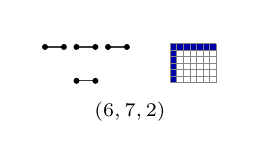
\begin{tikzpicture}[x=1mm,y=1mm,baseline=0mm]
\path[use as bounding box] (0,-1) rectangle (27,11);
\draw[black!78,line width=.43pt] (2.20,8.55)--(4.60,8.55);
\fill (2.20,8.55) circle[radius=.38mm];
\fill (4.60,8.55) circle[radius=.38mm];
\draw[black!78,line width=.43pt] (6.20,8.55)--(8.60,8.55);
\fill (6.20,8.55) circle[radius=.38mm];
\fill (8.60,8.55) circle[radius=.38mm];
\draw[black!78,line width=.43pt] (10.20,8.55)--(12.60,8.55);
\fill (10.20,8.55) circle[radius=.38mm];
\fill (12.60,8.55) circle[radius=.38mm];
\draw[black!78,line width=.43pt] (6.20,4.25)--(8.60,4.25);
\fill (6.20,4.25) circle[radius=.38mm];
\fill (8.60,4.25) circle[radius=.38mm];
\begin{scope}[shift={(18.095,4.010)},x=0.83mm,y=0.83mm]
\fill[blue!65!black] (0,0) rectangle (1,6) (0,5) rectangle (7,6);
\draw[black!48,line width=.16pt] (0,0)--(0,6) (1,0)--(1,6) (2,0)--(2,6) (3,0)--(3,6) (4,0)--(4,6) (5,0)--(5,6) (6,0)--(6,6) (7,0)--(7,6) (0,0)--(7,0) (0,1)--(7,1) (0,2)--(7,2) (0,3)--(7,3) (0,4)--(7,4) (0,5)--(7,5) (0,6)--(7,6);
\end{scope}
\node[font=\scriptsize,inner sep=0pt] at (13,.35) {$(6,7,2)$};
\end{tikzpicture} &
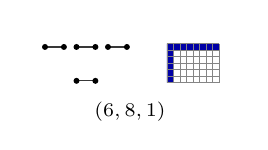
\begin{tikzpicture}[x=1mm,y=1mm,baseline=0mm]
\path[use as bounding box] (0,-1) rectangle (27,11);
\draw[black!78,line width=.43pt] (2.20,8.55)--(4.60,8.55);
\fill (2.20,8.55) circle[radius=.38mm];
\fill (4.60,8.55) circle[radius=.38mm];
\draw[black!78,line width=.43pt] (6.20,8.55)--(8.60,8.55);
\fill (6.20,8.55) circle[radius=.38mm];
\fill (8.60,8.55) circle[radius=.38mm];
\draw[black!78,line width=.43pt] (10.20,8.55)--(12.60,8.55);
\fill (10.20,8.55) circle[radius=.38mm];
\fill (12.60,8.55) circle[radius=.38mm];
\draw[black!78,line width=.43pt] (6.20,4.25)--(8.60,4.25);
\fill (6.20,4.25) circle[radius=.38mm];
\fill (8.60,4.25) circle[radius=.38mm];
\begin{scope}[shift={(17.680,4.010)},x=0.83mm,y=0.83mm]
\fill[blue!65!black] (0,0) rectangle (1,6) (0,5) rectangle (8,6);
\draw[black!48,line width=.16pt] (0,0)--(0,6) (1,0)--(1,6) (2,0)--(2,6) (3,0)--(3,6) (4,0)--(4,6) (5,0)--(5,6) (6,0)--(6,6) (7,0)--(7,6) (8,0)--(8,6) (0,0)--(8,0) (0,1)--(8,1) (0,2)--(8,2) (0,3)--(8,3) (0,4)--(8,4) (0,5)--(8,5) (0,6)--(8,6);
\end{scope}
\node[font=\scriptsize,inner sep=0pt] at (13,.35) {$(6,8,1)$};
\end{tikzpicture} &
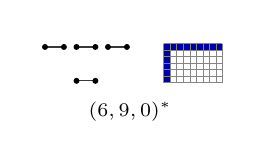
\begin{tikzpicture}[x=1mm,y=1mm,baseline=0mm]
\path[use as bounding box] (0,-1) rectangle (27,11);
\draw[black!78,line width=.43pt] (2.20,8.55)--(4.60,8.55);
\fill (2.20,8.55) circle[radius=.38mm];
\fill (4.60,8.55) circle[radius=.38mm];
\draw[black!78,line width=.43pt] (6.20,8.55)--(8.60,8.55);
\fill (6.20,8.55) circle[radius=.38mm];
\fill (8.60,8.55) circle[radius=.38mm];
\draw[black!78,line width=.43pt] (10.20,8.55)--(12.60,8.55);
\fill (10.20,8.55) circle[radius=.38mm];
\fill (12.60,8.55) circle[radius=.38mm];
\draw[black!78,line width=.43pt] (6.20,4.25)--(8.60,4.25);
\fill (6.20,4.25) circle[radius=.38mm];
\fill (8.60,4.25) circle[radius=.38mm];
\begin{scope}[shift={(17.265,4.010)},x=0.83mm,y=0.83mm]
\fill[blue!65!black] (0,0) rectangle (1,6) (0,5) rectangle (9,6);
\draw[black!48,line width=.16pt] (0,0)--(0,6) (1,0)--(1,6) (2,0)--(2,6) (3,0)--(3,6) (4,0)--(4,6) (5,0)--(5,6) (6,0)--(6,6) (7,0)--(7,6) (8,0)--(8,6) (9,0)--(9,6) (0,0)--(9,0) (0,1)--(9,1) (0,2)--(9,2) (0,3)--(9,3) (0,4)--(9,4) (0,5)--(9,5) (0,6)--(9,6);
\end{scope}
\node[font=\scriptsize,inner sep=0pt] at (13,.35) {$(6,9,0)^{*}$};
\end{tikzpicture} &
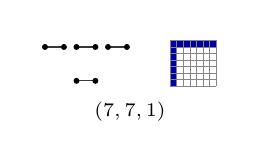
\begin{tikzpicture}[x=1mm,y=1mm,baseline=0mm]
\path[use as bounding box] (0,-1) rectangle (27,11);
\draw[black!78,line width=.43pt] (2.20,8.55)--(4.60,8.55);
\fill (2.20,8.55) circle[radius=.38mm];
\fill (4.60,8.55) circle[radius=.38mm];
\draw[black!78,line width=.43pt] (6.20,8.55)--(8.60,8.55);
\fill (6.20,8.55) circle[radius=.38mm];
\fill (8.60,8.55) circle[radius=.38mm];
\draw[black!78,line width=.43pt] (10.20,8.55)--(12.60,8.55);
\fill (10.20,8.55) circle[radius=.38mm];
\fill (12.60,8.55) circle[radius=.38mm];
\draw[black!78,line width=.43pt] (6.20,4.25)--(8.60,4.25);
\fill (6.20,4.25) circle[radius=.38mm];
\fill (8.60,4.25) circle[radius=.38mm];
\begin{scope}[shift={(18.095,3.595)},x=0.83mm,y=0.83mm]
\fill[blue!65!black] (0,0) rectangle (1,7) (0,6) rectangle (7,7);
\draw[black!48,line width=.16pt] (0,0)--(0,7) (1,0)--(1,7) (2,0)--(2,7) (3,0)--(3,7) (4,0)--(4,7) (5,0)--(5,7) (6,0)--(6,7) (7,0)--(7,7) (0,0)--(7,0) (0,1)--(7,1) (0,2)--(7,2) (0,3)--(7,3) (0,4)--(7,4) (0,5)--(7,5) (0,6)--(7,6) (0,7)--(7,7);
\end{scope}
\node[font=\scriptsize,inner sep=0pt] at (13,.35) {$(7,7,1)$};
\end{tikzpicture} \\[.5mm]
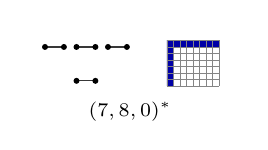
\begin{tikzpicture}[x=1mm,y=1mm,baseline=0mm]
\path[use as bounding box] (0,-1) rectangle (27,11);
\draw[black!78,line width=.43pt] (2.20,8.55)--(4.60,8.55);
\fill (2.20,8.55) circle[radius=.38mm];
\fill (4.60,8.55) circle[radius=.38mm];
\draw[black!78,line width=.43pt] (6.20,8.55)--(8.60,8.55);
\fill (6.20,8.55) circle[radius=.38mm];
\fill (8.60,8.55) circle[radius=.38mm];
\draw[black!78,line width=.43pt] (10.20,8.55)--(12.60,8.55);
\fill (10.20,8.55) circle[radius=.38mm];
\fill (12.60,8.55) circle[radius=.38mm];
\draw[black!78,line width=.43pt] (6.20,4.25)--(8.60,4.25);
\fill (6.20,4.25) circle[radius=.38mm];
\fill (8.60,4.25) circle[radius=.38mm];
\begin{scope}[shift={(17.680,3.595)},x=0.83mm,y=0.83mm]
\fill[blue!65!black] (0,0) rectangle (1,7) (0,6) rectangle (8,7);
\draw[black!48,line width=.16pt] (0,0)--(0,7) (1,0)--(1,7) (2,0)--(2,7) (3,0)--(3,7) (4,0)--(4,7) (5,0)--(5,7) (6,0)--(6,7) (7,0)--(7,7) (8,0)--(8,7) (0,0)--(8,0) (0,1)--(8,1) (0,2)--(8,2) (0,3)--(8,3) (0,4)--(8,4) (0,5)--(8,5) (0,6)--(8,6) (0,7)--(8,7);
\end{scope}
\node[font=\scriptsize,inner sep=0pt] at (13,.35) {$(7,8,0)^{*}$};
\end{tikzpicture} \\[.5mm]
\end{tabular}
\caption{Order-23 templates with 4 unmarked edges. Starred templates also occur in the triangle-free list.}
\label{fig:nine-chain-2}
\end{figure}

\begin{figure}[!htbp]
\centering
\begin{tabular}{@{}c@{\hspace{2.5mm}}c@{\hspace{2.5mm}}c@{\hspace{2.5mm}}c@{}}
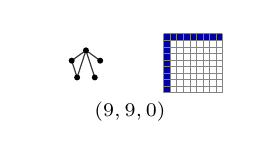
\begin{tikzpicture}[x=1mm,y=1mm,baseline=0mm]
\path[use as bounding box] (0,-1) rectangle (27,11);
\draw[black!78,line width=.43pt] (7.40,8.12)--(5.59,6.81) (7.40,8.12)--(6.28,4.68) (7.40,8.12)--(8.52,4.68) (7.40,8.12)--(9.21,6.81) (5.59,6.81)--(6.28,4.68);
\fill (7.40,8.12) circle[radius=.38mm];
\fill (5.59,6.81) circle[radius=.38mm];
\fill (6.28,4.68) circle[radius=.38mm];
\fill (8.52,4.68) circle[radius=.38mm];
\fill (9.21,6.81) circle[radius=.38mm];
\begin{scope}[shift={(17.265,2.765)},x=0.83mm,y=0.83mm]
\fill[blue!65!black] (0,0) rectangle (1,9) (0,8) rectangle (9,9);
\draw[black!48,line width=.16pt] (0,0)--(0,9) (1,0)--(1,9) (2,0)--(2,9) (3,0)--(3,9) (4,0)--(4,9) (5,0)--(5,9) (6,0)--(6,9) (7,0)--(7,9) (8,0)--(8,9) (9,0)--(9,9) (0,0)--(9,0) (0,1)--(9,1) (0,2)--(9,2) (0,3)--(9,3) (0,4)--(9,4) (0,5)--(9,5) (0,6)--(9,6) (0,7)--(9,7) (0,8)--(9,8) (0,9)--(9,9);
\end{scope}
\node[font=\scriptsize,inner sep=0pt] at (13,.35) {$(9,9,0)$};
\end{tikzpicture} &
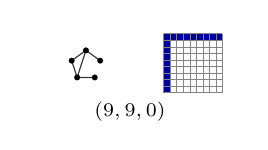
\begin{tikzpicture}[x=1mm,y=1mm,baseline=0mm]
\path[use as bounding box] (0,-1) rectangle (27,11);
\draw[black!78,line width=.43pt] (7.40,8.12)--(6.28,4.68) (7.40,8.12)--(5.59,6.81) (7.40,8.12)--(9.21,6.81) (6.28,4.68)--(5.59,6.81) (6.28,4.68)--(8.52,4.68);
\fill (7.40,8.12) circle[radius=.38mm];
\fill (6.28,4.68) circle[radius=.38mm];
\fill (5.59,6.81) circle[radius=.38mm];
\fill (9.21,6.81) circle[radius=.38mm];
\fill (8.52,4.68) circle[radius=.38mm];
\begin{scope}[shift={(17.265,2.765)},x=0.83mm,y=0.83mm]
\fill[blue!65!black] (0,0) rectangle (1,9) (0,8) rectangle (9,9);
\draw[black!48,line width=.16pt] (0,0)--(0,9) (1,0)--(1,9) (2,0)--(2,9) (3,0)--(3,9) (4,0)--(4,9) (5,0)--(5,9) (6,0)--(6,9) (7,0)--(7,9) (8,0)--(8,9) (9,0)--(9,9) (0,0)--(9,0) (0,1)--(9,1) (0,2)--(9,2) (0,3)--(9,3) (0,4)--(9,4) (0,5)--(9,5) (0,6)--(9,6) (0,7)--(9,7) (0,8)--(9,8) (0,9)--(9,9);
\end{scope}
\node[font=\scriptsize,inner sep=0pt] at (13,.35) {$(9,9,0)$};
\end{tikzpicture} &
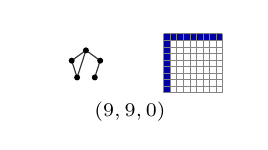
\begin{tikzpicture}[x=1mm,y=1mm,baseline=0mm]
\path[use as bounding box] (0,-1) rectangle (27,11);
\draw[black!78,line width=.43pt] (7.40,8.12)--(5.59,6.81) (7.40,8.12)--(6.28,4.68) (7.40,8.12)--(9.21,6.81) (5.59,6.81)--(6.28,4.68) (9.21,6.81)--(8.52,4.68);
\fill (7.40,8.12) circle[radius=.38mm];
\fill (5.59,6.81) circle[radius=.38mm];
\fill (6.28,4.68) circle[radius=.38mm];
\fill (9.21,6.81) circle[radius=.38mm];
\fill (8.52,4.68) circle[radius=.38mm];
\begin{scope}[shift={(17.265,2.765)},x=0.83mm,y=0.83mm]
\fill[blue!65!black] (0,0) rectangle (1,9) (0,8) rectangle (9,9);
\draw[black!48,line width=.16pt] (0,0)--(0,9) (1,0)--(1,9) (2,0)--(2,9) (3,0)--(3,9) (4,0)--(4,9) (5,0)--(5,9) (6,0)--(6,9) (7,0)--(7,9) (8,0)--(8,9) (9,0)--(9,9) (0,0)--(9,0) (0,1)--(9,1) (0,2)--(9,2) (0,3)--(9,3) (0,4)--(9,4) (0,5)--(9,5) (0,6)--(9,6) (0,7)--(9,7) (0,8)--(9,8) (0,9)--(9,9);
\end{scope}
\node[font=\scriptsize,inner sep=0pt] at (13,.35) {$(9,9,0)$};
\end{tikzpicture} &
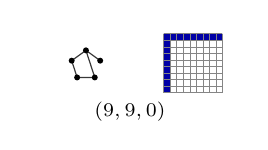
\begin{tikzpicture}[x=1mm,y=1mm,baseline=0mm]
\path[use as bounding box] (0,-1) rectangle (27,11);
\draw[black!78,line width=.43pt] (7.40,8.12)--(5.59,6.81) (7.40,8.12)--(8.52,4.68) (7.40,8.12)--(9.21,6.81) (5.59,6.81)--(6.28,4.68) (8.52,4.68)--(6.28,4.68);
\fill (7.40,8.12) circle[radius=.38mm];
\fill (5.59,6.81) circle[radius=.38mm];
\fill (8.52,4.68) circle[radius=.38mm];
\fill (6.28,4.68) circle[radius=.38mm];
\fill (9.21,6.81) circle[radius=.38mm];
\begin{scope}[shift={(17.265,2.765)},x=0.83mm,y=0.83mm]
\fill[blue!65!black] (0,0) rectangle (1,9) (0,8) rectangle (9,9);
\draw[black!48,line width=.16pt] (0,0)--(0,9) (1,0)--(1,9) (2,0)--(2,9) (3,0)--(3,9) (4,0)--(4,9) (5,0)--(5,9) (6,0)--(6,9) (7,0)--(7,9) (8,0)--(8,9) (9,0)--(9,9) (0,0)--(9,0) (0,1)--(9,1) (0,2)--(9,2) (0,3)--(9,3) (0,4)--(9,4) (0,5)--(9,5) (0,6)--(9,6) (0,7)--(9,7) (0,8)--(9,8) (0,9)--(9,9);
\end{scope}
\node[font=\scriptsize,inner sep=0pt] at (13,.35) {$(9,9,0)$};
\end{tikzpicture} \\[.5mm]
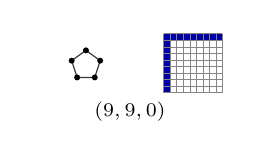
\begin{tikzpicture}[x=1mm,y=1mm,baseline=0mm]
\path[use as bounding box] (0,-1) rectangle (27,11);
\draw[black!78,line width=.43pt] (7.40,8.12)--(5.59,6.81) (7.40,8.12)--(9.21,6.81) (5.59,6.81)--(6.28,4.68) (9.21,6.81)--(8.52,4.68) (6.28,4.68)--(8.52,4.68);
\fill (7.40,8.12) circle[radius=.38mm];
\fill (5.59,6.81) circle[radius=.38mm];
\fill (9.21,6.81) circle[radius=.38mm];
\fill (6.28,4.68) circle[radius=.38mm];
\fill (8.52,4.68) circle[radius=.38mm];
\begin{scope}[shift={(17.265,2.765)},x=0.83mm,y=0.83mm]
\fill[blue!65!black] (0,0) rectangle (1,9) (0,8) rectangle (9,9);
\draw[black!48,line width=.16pt] (0,0)--(0,9) (1,0)--(1,9) (2,0)--(2,9) (3,0)--(3,9) (4,0)--(4,9) (5,0)--(5,9) (6,0)--(6,9) (7,0)--(7,9) (8,0)--(8,9) (9,0)--(9,9) (0,0)--(9,0) (0,1)--(9,1) (0,2)--(9,2) (0,3)--(9,3) (0,4)--(9,4) (0,5)--(9,5) (0,6)--(9,6) (0,7)--(9,7) (0,8)--(9,8) (0,9)--(9,9);
\end{scope}
\node[font=\scriptsize,inner sep=0pt] at (13,.35) {$(9,9,0)$};
\end{tikzpicture} &
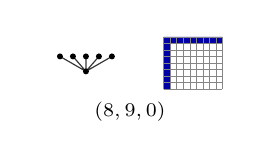
\begin{tikzpicture}[x=1mm,y=1mm,baseline=0mm]
\path[use as bounding box] (0,-1) rectangle (27,11);
\draw[black!78,line width=.43pt] (7.40,5.45)--(4.10,7.35) (7.40,5.45)--(5.75,7.35) (7.40,5.45)--(7.40,7.35) (7.40,5.45)--(9.05,7.35) (7.40,5.45)--(10.70,7.35);
\fill (7.40,5.45) circle[radius=.38mm];
\fill (4.10,7.35) circle[radius=.38mm];
\fill (5.75,7.35) circle[radius=.38mm];
\fill (7.40,7.35) circle[radius=.38mm];
\fill (9.05,7.35) circle[radius=.38mm];
\fill (10.70,7.35) circle[radius=.38mm];
\begin{scope}[shift={(17.265,3.180)},x=0.83mm,y=0.83mm]
\fill[blue!65!black] (0,0) rectangle (1,8) (0,7) rectangle (9,8);
\draw[black!48,line width=.16pt] (0,0)--(0,8) (1,0)--(1,8) (2,0)--(2,8) (3,0)--(3,8) (4,0)--(4,8) (5,0)--(5,8) (6,0)--(6,8) (7,0)--(7,8) (8,0)--(8,8) (9,0)--(9,8) (0,0)--(9,0) (0,1)--(9,1) (0,2)--(9,2) (0,3)--(9,3) (0,4)--(9,4) (0,5)--(9,5) (0,6)--(9,6) (0,7)--(9,7) (0,8)--(9,8);
\end{scope}
\node[font=\scriptsize,inner sep=0pt] at (13,.35) {$(8,9,0)$};
\end{tikzpicture} &
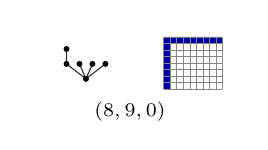
\begin{tikzpicture}[x=1mm,y=1mm,baseline=0mm]
\path[use as bounding box] (0,-1) rectangle (27,11);
\draw[black!78,line width=.43pt] (7.40,4.50)--(4.93,6.40) (7.40,4.50)--(6.58,6.40) (7.40,4.50)--(8.23,6.40) (7.40,4.50)--(9.88,6.40) (4.93,6.40)--(4.93,8.30);
\fill (7.40,4.50) circle[radius=.38mm];
\fill (4.93,6.40) circle[radius=.38mm];
\fill (6.58,6.40) circle[radius=.38mm];
\fill (8.23,6.40) circle[radius=.38mm];
\fill (9.88,6.40) circle[radius=.38mm];
\fill (4.93,8.30) circle[radius=.38mm];
\begin{scope}[shift={(17.265,3.180)},x=0.83mm,y=0.83mm]
\fill[blue!65!black] (0,0) rectangle (1,8) (0,7) rectangle (9,8);
\draw[black!48,line width=.16pt] (0,0)--(0,8) (1,0)--(1,8) (2,0)--(2,8) (3,0)--(3,8) (4,0)--(4,8) (5,0)--(5,8) (6,0)--(6,8) (7,0)--(7,8) (8,0)--(8,8) (9,0)--(9,8) (0,0)--(9,0) (0,1)--(9,1) (0,2)--(9,2) (0,3)--(9,3) (0,4)--(9,4) (0,5)--(9,5) (0,6)--(9,6) (0,7)--(9,7) (0,8)--(9,8);
\end{scope}
\node[font=\scriptsize,inner sep=0pt] at (13,.35) {$(8,9,0)$};
\end{tikzpicture} &
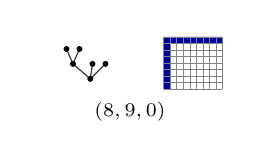
\begin{tikzpicture}[x=1mm,y=1mm,baseline=0mm]
\path[use as bounding box] (0,-1) rectangle (27,11);
\draw[black!78,line width=.43pt] (7.95,4.50)--(5.75,6.40) (7.95,4.50)--(8.23,6.40) (7.95,4.50)--(9.88,6.40) (5.75,6.40)--(4.93,8.30) (5.75,6.40)--(6.58,8.30);
\fill (7.95,4.50) circle[radius=.38mm];
\fill (5.75,6.40) circle[radius=.38mm];
\fill (8.23,6.40) circle[radius=.38mm];
\fill (9.88,6.40) circle[radius=.38mm];
\fill (4.93,8.30) circle[radius=.38mm];
\fill (6.58,8.30) circle[radius=.38mm];
\begin{scope}[shift={(17.265,3.180)},x=0.83mm,y=0.83mm]
\fill[blue!65!black] (0,0) rectangle (1,8) (0,7) rectangle (9,8);
\draw[black!48,line width=.16pt] (0,0)--(0,8) (1,0)--(1,8) (2,0)--(2,8) (3,0)--(3,8) (4,0)--(4,8) (5,0)--(5,8) (6,0)--(6,8) (7,0)--(7,8) (8,0)--(8,8) (9,0)--(9,8) (0,0)--(9,0) (0,1)--(9,1) (0,2)--(9,2) (0,3)--(9,3) (0,4)--(9,4) (0,5)--(9,5) (0,6)--(9,6) (0,7)--(9,7) (0,8)--(9,8);
\end{scope}
\node[font=\scriptsize,inner sep=0pt] at (13,.35) {$(8,9,0)$};
\end{tikzpicture} \\[.5mm]
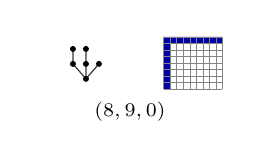
\begin{tikzpicture}[x=1mm,y=1mm,baseline=0mm]
\path[use as bounding box] (0,-1) rectangle (27,11);
\draw[black!78,line width=.43pt] (7.40,4.50)--(5.75,6.40) (7.40,4.50)--(7.40,6.40) (7.40,4.50)--(9.05,6.40) (5.75,6.40)--(5.75,8.30) (7.40,6.40)--(7.40,8.30);
\fill (7.40,4.50) circle[radius=.38mm];
\fill (5.75,6.40) circle[radius=.38mm];
\fill (7.40,6.40) circle[radius=.38mm];
\fill (9.05,6.40) circle[radius=.38mm];
\fill (5.75,8.30) circle[radius=.38mm];
\fill (7.40,8.30) circle[radius=.38mm];
\begin{scope}[shift={(17.265,3.180)},x=0.83mm,y=0.83mm]
\fill[blue!65!black] (0,0) rectangle (1,8) (0,7) rectangle (9,8);
\draw[black!48,line width=.16pt] (0,0)--(0,8) (1,0)--(1,8) (2,0)--(2,8) (3,0)--(3,8) (4,0)--(4,8) (5,0)--(5,8) (6,0)--(6,8) (7,0)--(7,8) (8,0)--(8,8) (9,0)--(9,8) (0,0)--(9,0) (0,1)--(9,1) (0,2)--(9,2) (0,3)--(9,3) (0,4)--(9,4) (0,5)--(9,5) (0,6)--(9,6) (0,7)--(9,7) (0,8)--(9,8);
\end{scope}
\node[font=\scriptsize,inner sep=0pt] at (13,.35) {$(8,9,0)$};
\end{tikzpicture} &
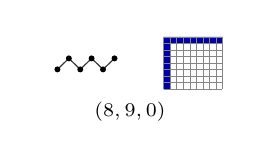
\begin{tikzpicture}[x=1mm,y=1mm,baseline=0mm]
\path[use as bounding box] (0,-1) rectangle (27,11);
\draw[black!78,line width=.43pt] (6.68,5.70)--(8.12,7.10) (6.68,5.70)--(5.23,7.10) (8.12,7.10)--(9.57,5.70) (5.23,7.10)--(3.78,5.70) (9.57,5.70)--(11.03,7.10);
\fill (6.68,5.70) circle[radius=.38mm];
\fill (8.12,7.10) circle[radius=.38mm];
\fill (5.23,7.10) circle[radius=.38mm];
\fill (9.57,5.70) circle[radius=.38mm];
\fill (3.78,5.70) circle[radius=.38mm];
\fill (11.03,7.10) circle[radius=.38mm];
\begin{scope}[shift={(17.265,3.180)},x=0.83mm,y=0.83mm]
\fill[blue!65!black] (0,0) rectangle (1,8) (0,7) rectangle (9,8);
\draw[black!48,line width=.16pt] (0,0)--(0,8) (1,0)--(1,8) (2,0)--(2,8) (3,0)--(3,8) (4,0)--(4,8) (5,0)--(5,8) (6,0)--(6,8) (7,0)--(7,8) (8,0)--(8,8) (9,0)--(9,8) (0,0)--(9,0) (0,1)--(9,1) (0,2)--(9,2) (0,3)--(9,3) (0,4)--(9,4) (0,5)--(9,5) (0,6)--(9,6) (0,7)--(9,7) (0,8)--(9,8);
\end{scope}
\node[font=\scriptsize,inner sep=0pt] at (13,.35) {$(8,9,0)$};
\end{tikzpicture} &
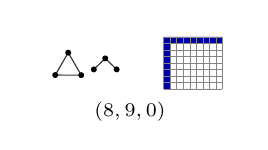
\begin{tikzpicture}[x=1mm,y=1mm,baseline=0mm]
\path[use as bounding box] (0,-1) rectangle (27,11);
\draw[black!78,line width=.43pt] (5.15,7.83)--(3.50,4.98) (5.15,7.83)--(6.80,4.97) (3.50,4.98)--(6.80,4.97);
\fill (5.15,7.83) circle[radius=.38mm];
\fill (3.50,4.98) circle[radius=.38mm];
\fill (6.80,4.97) circle[radius=.38mm];
\draw[black!78,line width=.43pt] (9.85,7.10)--(8.40,5.70) (9.85,7.10)--(11.30,5.70);
\fill (9.85,7.10) circle[radius=.38mm];
\fill (8.40,5.70) circle[radius=.38mm];
\fill (11.30,5.70) circle[radius=.38mm];
\begin{scope}[shift={(17.265,3.180)},x=0.83mm,y=0.83mm]
\fill[blue!65!black] (0,0) rectangle (1,8) (0,7) rectangle (9,8);
\draw[black!48,line width=.16pt] (0,0)--(0,8) (1,0)--(1,8) (2,0)--(2,8) (3,0)--(3,8) (4,0)--(4,8) (5,0)--(5,8) (6,0)--(6,8) (7,0)--(7,8) (8,0)--(8,8) (9,0)--(9,8) (0,0)--(9,0) (0,1)--(9,1) (0,2)--(9,2) (0,3)--(9,3) (0,4)--(9,4) (0,5)--(9,5) (0,6)--(9,6) (0,7)--(9,7) (0,8)--(9,8);
\end{scope}
\node[font=\scriptsize,inner sep=0pt] at (13,.35) {$(8,9,0)$};
\end{tikzpicture} &
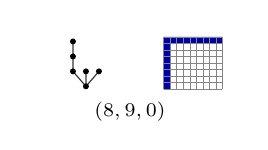
\begin{tikzpicture}[x=1mm,y=1mm,baseline=0mm]
\path[use as bounding box] (0,-1) rectangle (27,11);
\draw[black!78,line width=.43pt] (7.40,3.55)--(5.75,5.45) (7.40,3.55)--(7.40,5.45) (7.40,3.55)--(9.05,5.45) (5.75,5.45)--(5.75,7.35) (5.75,7.35)--(5.75,9.25);
\fill (7.40,3.55) circle[radius=.38mm];
\fill (5.75,5.45) circle[radius=.38mm];
\fill (5.75,7.35) circle[radius=.38mm];
\fill (7.40,5.45) circle[radius=.38mm];
\fill (9.05,5.45) circle[radius=.38mm];
\fill (5.75,9.25) circle[radius=.38mm];
\begin{scope}[shift={(17.265,3.180)},x=0.83mm,y=0.83mm]
\fill[blue!65!black] (0,0) rectangle (1,8) (0,7) rectangle (9,8);
\draw[black!48,line width=.16pt] (0,0)--(0,8) (1,0)--(1,8) (2,0)--(2,8) (3,0)--(3,8) (4,0)--(4,8) (5,0)--(5,8) (6,0)--(6,8) (7,0)--(7,8) (8,0)--(8,8) (9,0)--(9,8) (0,0)--(9,0) (0,1)--(9,1) (0,2)--(9,2) (0,3)--(9,3) (0,4)--(9,4) (0,5)--(9,5) (0,6)--(9,6) (0,7)--(9,7) (0,8)--(9,8);
\end{scope}
\node[font=\scriptsize,inner sep=0pt] at (13,.35) {$(8,9,0)$};
\end{tikzpicture} \\[.5mm]
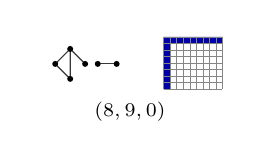
\begin{tikzpicture}[x=1mm,y=1mm,baseline=0mm]
\path[use as bounding box] (0,-1) rectangle (27,11);
\draw[black!78,line width=.43pt] (5.40,8.30)--(3.50,6.40) (5.40,8.30)--(5.40,4.50) (5.40,8.30)--(7.30,6.40) (3.50,6.40)--(5.40,4.50);
\fill (5.40,8.30) circle[radius=.38mm];
\fill (3.50,6.40) circle[radius=.38mm];
\fill (5.40,4.50) circle[radius=.38mm];
\fill (7.30,6.40) circle[radius=.38mm];
\draw[black!78,line width=.43pt] (8.90,6.40)--(11.30,6.40);
\fill (8.90,6.40) circle[radius=.38mm];
\fill (11.30,6.40) circle[radius=.38mm];
\begin{scope}[shift={(17.265,3.180)},x=0.83mm,y=0.83mm]
\fill[blue!65!black] (0,0) rectangle (1,8) (0,7) rectangle (9,8);
\draw[black!48,line width=.16pt] (0,0)--(0,8) (1,0)--(1,8) (2,0)--(2,8) (3,0)--(3,8) (4,0)--(4,8) (5,0)--(5,8) (6,0)--(6,8) (7,0)--(7,8) (8,0)--(8,8) (9,0)--(9,8) (0,0)--(9,0) (0,1)--(9,1) (0,2)--(9,2) (0,3)--(9,3) (0,4)--(9,4) (0,5)--(9,5) (0,6)--(9,6) (0,7)--(9,7) (0,8)--(9,8);
\end{scope}
\node[font=\scriptsize,inner sep=0pt] at (13,.35) {$(8,9,0)$};
\end{tikzpicture} &
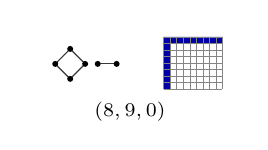
\begin{tikzpicture}[x=1mm,y=1mm,baseline=0mm]
\path[use as bounding box] (0,-1) rectangle (27,11);
\draw[black!78,line width=.43pt] (5.40,8.30)--(3.50,6.40) (5.40,8.30)--(7.30,6.40) (3.50,6.40)--(5.40,4.50) (7.30,6.40)--(5.40,4.50);
\fill (5.40,8.30) circle[radius=.38mm];
\fill (3.50,6.40) circle[radius=.38mm];
\fill (7.30,6.40) circle[radius=.38mm];
\fill (5.40,4.50) circle[radius=.38mm];
\draw[black!78,line width=.43pt] (8.90,6.40)--(11.30,6.40);
\fill (8.90,6.40) circle[radius=.38mm];
\fill (11.30,6.40) circle[radius=.38mm];
\begin{scope}[shift={(17.265,3.180)},x=0.83mm,y=0.83mm]
\fill[blue!65!black] (0,0) rectangle (1,8) (0,7) rectangle (9,8);
\draw[black!48,line width=.16pt] (0,0)--(0,8) (1,0)--(1,8) (2,0)--(2,8) (3,0)--(3,8) (4,0)--(4,8) (5,0)--(5,8) (6,0)--(6,8) (7,0)--(7,8) (8,0)--(8,8) (9,0)--(9,8) (0,0)--(9,0) (0,1)--(9,1) (0,2)--(9,2) (0,3)--(9,3) (0,4)--(9,4) (0,5)--(9,5) (0,6)--(9,6) (0,7)--(9,7) (0,8)--(9,8);
\end{scope}
\node[font=\scriptsize,inner sep=0pt] at (13,.35) {$(8,9,0)$};
\end{tikzpicture} &
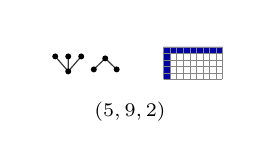
\begin{tikzpicture}[x=1mm,y=1mm,baseline=0mm]
\path[use as bounding box] (0,-1) rectangle (27,11);
\draw[black!78,line width=.43pt] (5.15,5.45)--(3.50,7.35) (5.15,5.45)--(5.15,7.35) (5.15,5.45)--(6.80,7.35);
\fill (5.15,5.45) circle[radius=.38mm];
\fill (3.50,7.35) circle[radius=.38mm];
\fill (5.15,7.35) circle[radius=.38mm];
\fill (6.80,7.35) circle[radius=.38mm];
\draw[black!78,line width=.43pt] (9.85,7.10)--(8.40,5.70) (9.85,7.10)--(11.30,5.70);
\fill (9.85,7.10) circle[radius=.38mm];
\fill (8.40,5.70) circle[radius=.38mm];
\fill (11.30,5.70) circle[radius=.38mm];
\begin{scope}[shift={(17.265,4.425)},x=0.83mm,y=0.83mm]
\fill[blue!65!black] (0,0) rectangle (1,5) (0,4) rectangle (9,5);
\draw[black!48,line width=.16pt] (0,0)--(0,5) (1,0)--(1,5) (2,0)--(2,5) (3,0)--(3,5) (4,0)--(4,5) (5,0)--(5,5) (6,0)--(6,5) (7,0)--(7,5) (8,0)--(8,5) (9,0)--(9,5) (0,0)--(9,0) (0,1)--(9,1) (0,2)--(9,2) (0,3)--(9,3) (0,4)--(9,4) (0,5)--(9,5);
\end{scope}
\node[font=\scriptsize,inner sep=0pt] at (13,.35) {$(5,9,2)$};
\end{tikzpicture} &
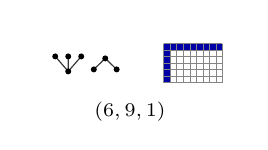
\begin{tikzpicture}[x=1mm,y=1mm,baseline=0mm]
\path[use as bounding box] (0,-1) rectangle (27,11);
\draw[black!78,line width=.43pt] (5.15,5.45)--(3.50,7.35) (5.15,5.45)--(5.15,7.35) (5.15,5.45)--(6.80,7.35);
\fill (5.15,5.45) circle[radius=.38mm];
\fill (3.50,7.35) circle[radius=.38mm];
\fill (5.15,7.35) circle[radius=.38mm];
\fill (6.80,7.35) circle[radius=.38mm];
\draw[black!78,line width=.43pt] (9.85,7.10)--(8.40,5.70) (9.85,7.10)--(11.30,5.70);
\fill (9.85,7.10) circle[radius=.38mm];
\fill (8.40,5.70) circle[radius=.38mm];
\fill (11.30,5.70) circle[radius=.38mm];
\begin{scope}[shift={(17.265,4.010)},x=0.83mm,y=0.83mm]
\fill[blue!65!black] (0,0) rectangle (1,6) (0,5) rectangle (9,6);
\draw[black!48,line width=.16pt] (0,0)--(0,6) (1,0)--(1,6) (2,0)--(2,6) (3,0)--(3,6) (4,0)--(4,6) (5,0)--(5,6) (6,0)--(6,6) (7,0)--(7,6) (8,0)--(8,6) (9,0)--(9,6) (0,0)--(9,0) (0,1)--(9,1) (0,2)--(9,2) (0,3)--(9,3) (0,4)--(9,4) (0,5)--(9,5) (0,6)--(9,6);
\end{scope}
\node[font=\scriptsize,inner sep=0pt] at (13,.35) {$(6,9,1)$};
\end{tikzpicture} \\[.5mm]
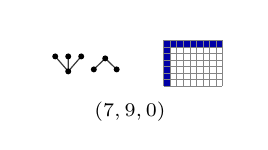
\begin{tikzpicture}[x=1mm,y=1mm,baseline=0mm]
\path[use as bounding box] (0,-1) rectangle (27,11);
\draw[black!78,line width=.43pt] (5.15,5.45)--(3.50,7.35) (5.15,5.45)--(5.15,7.35) (5.15,5.45)--(6.80,7.35);
\fill (5.15,5.45) circle[radius=.38mm];
\fill (3.50,7.35) circle[radius=.38mm];
\fill (5.15,7.35) circle[radius=.38mm];
\fill (6.80,7.35) circle[radius=.38mm];
\draw[black!78,line width=.43pt] (9.85,7.10)--(8.40,5.70) (9.85,7.10)--(11.30,5.70);
\fill (9.85,7.10) circle[radius=.38mm];
\fill (8.40,5.70) circle[radius=.38mm];
\fill (11.30,5.70) circle[radius=.38mm];
\begin{scope}[shift={(17.265,3.595)},x=0.83mm,y=0.83mm]
\fill[blue!65!black] (0,0) rectangle (1,7) (0,6) rectangle (9,7);
\draw[black!48,line width=.16pt] (0,0)--(0,7) (1,0)--(1,7) (2,0)--(2,7) (3,0)--(3,7) (4,0)--(4,7) (5,0)--(5,7) (6,0)--(6,7) (7,0)--(7,7) (8,0)--(8,7) (9,0)--(9,7) (0,0)--(9,0) (0,1)--(9,1) (0,2)--(9,2) (0,3)--(9,3) (0,4)--(9,4) (0,5)--(9,5) (0,6)--(9,6) (0,7)--(9,7);
\end{scope}
\node[font=\scriptsize,inner sep=0pt] at (13,.35) {$(7,9,0)$};
\end{tikzpicture} &
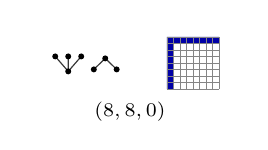
\begin{tikzpicture}[x=1mm,y=1mm,baseline=0mm]
\path[use as bounding box] (0,-1) rectangle (27,11);
\draw[black!78,line width=.43pt] (5.15,5.45)--(3.50,7.35) (5.15,5.45)--(5.15,7.35) (5.15,5.45)--(6.80,7.35);
\fill (5.15,5.45) circle[radius=.38mm];
\fill (3.50,7.35) circle[radius=.38mm];
\fill (5.15,7.35) circle[radius=.38mm];
\fill (6.80,7.35) circle[radius=.38mm];
\draw[black!78,line width=.43pt] (9.85,7.10)--(8.40,5.70) (9.85,7.10)--(11.30,5.70);
\fill (9.85,7.10) circle[radius=.38mm];
\fill (8.40,5.70) circle[radius=.38mm];
\fill (11.30,5.70) circle[radius=.38mm];
\begin{scope}[shift={(17.680,3.180)},x=0.83mm,y=0.83mm]
\fill[blue!65!black] (0,0) rectangle (1,8) (0,7) rectangle (8,8);
\draw[black!48,line width=.16pt] (0,0)--(0,8) (1,0)--(1,8) (2,0)--(2,8) (3,0)--(3,8) (4,0)--(4,8) (5,0)--(5,8) (6,0)--(6,8) (7,0)--(7,8) (8,0)--(8,8) (0,0)--(8,0) (0,1)--(8,1) (0,2)--(8,2) (0,3)--(8,3) (0,4)--(8,4) (0,5)--(8,5) (0,6)--(8,6) (0,7)--(8,7) (0,8)--(8,8);
\end{scope}
\node[font=\scriptsize,inner sep=0pt] at (13,.35) {$(8,8,0)$};
\end{tikzpicture} &
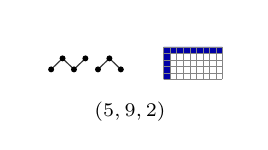
\begin{tikzpicture}[x=1mm,y=1mm,baseline=0mm]
\path[use as bounding box] (0,-1) rectangle (27,11);
\draw[black!78,line width=.43pt] (4.43,7.10)--(5.88,5.70) (4.43,7.10)--(2.98,5.70) (5.88,5.70)--(7.33,7.10);
\fill (4.43,7.10) circle[radius=.38mm];
\fill (5.88,5.70) circle[radius=.38mm];
\fill (2.98,5.70) circle[radius=.38mm];
\fill (7.33,7.10) circle[radius=.38mm];
\draw[black!78,line width=.43pt] (10.38,7.10)--(8.93,5.70) (10.38,7.10)--(11.83,5.70);
\fill (10.38,7.10) circle[radius=.38mm];
\fill (8.93,5.70) circle[radius=.38mm];
\fill (11.83,5.70) circle[radius=.38mm];
\begin{scope}[shift={(17.265,4.425)},x=0.83mm,y=0.83mm]
\fill[blue!65!black] (0,0) rectangle (1,5) (0,4) rectangle (9,5);
\draw[black!48,line width=.16pt] (0,0)--(0,5) (1,0)--(1,5) (2,0)--(2,5) (3,0)--(3,5) (4,0)--(4,5) (5,0)--(5,5) (6,0)--(6,5) (7,0)--(7,5) (8,0)--(8,5) (9,0)--(9,5) (0,0)--(9,0) (0,1)--(9,1) (0,2)--(9,2) (0,3)--(9,3) (0,4)--(9,4) (0,5)--(9,5);
\end{scope}
\node[font=\scriptsize,inner sep=0pt] at (13,.35) {$(5,9,2)$};
\end{tikzpicture} &
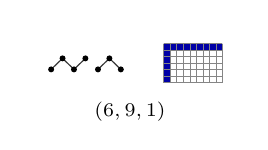
\begin{tikzpicture}[x=1mm,y=1mm,baseline=0mm]
\path[use as bounding box] (0,-1) rectangle (27,11);
\draw[black!78,line width=.43pt] (4.43,7.10)--(5.88,5.70) (4.43,7.10)--(2.98,5.70) (5.88,5.70)--(7.33,7.10);
\fill (4.43,7.10) circle[radius=.38mm];
\fill (5.88,5.70) circle[radius=.38mm];
\fill (2.98,5.70) circle[radius=.38mm];
\fill (7.33,7.10) circle[radius=.38mm];
\draw[black!78,line width=.43pt] (10.38,7.10)--(8.93,5.70) (10.38,7.10)--(11.83,5.70);
\fill (10.38,7.10) circle[radius=.38mm];
\fill (8.93,5.70) circle[radius=.38mm];
\fill (11.83,5.70) circle[radius=.38mm];
\begin{scope}[shift={(17.265,4.010)},x=0.83mm,y=0.83mm]
\fill[blue!65!black] (0,0) rectangle (1,6) (0,5) rectangle (9,6);
\draw[black!48,line width=.16pt] (0,0)--(0,6) (1,0)--(1,6) (2,0)--(2,6) (3,0)--(3,6) (4,0)--(4,6) (5,0)--(5,6) (6,0)--(6,6) (7,0)--(7,6) (8,0)--(8,6) (9,0)--(9,6) (0,0)--(9,0) (0,1)--(9,1) (0,2)--(9,2) (0,3)--(9,3) (0,4)--(9,4) (0,5)--(9,5) (0,6)--(9,6);
\end{scope}
\node[font=\scriptsize,inner sep=0pt] at (13,.35) {$(6,9,1)$};
\end{tikzpicture} \\[.5mm]
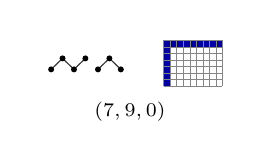
\begin{tikzpicture}[x=1mm,y=1mm,baseline=0mm]
\path[use as bounding box] (0,-1) rectangle (27,11);
\draw[black!78,line width=.43pt] (4.43,7.10)--(5.88,5.70) (4.43,7.10)--(2.98,5.70) (5.88,5.70)--(7.33,7.10);
\fill (4.43,7.10) circle[radius=.38mm];
\fill (5.88,5.70) circle[radius=.38mm];
\fill (2.98,5.70) circle[radius=.38mm];
\fill (7.33,7.10) circle[radius=.38mm];
\draw[black!78,line width=.43pt] (10.38,7.10)--(8.93,5.70) (10.38,7.10)--(11.83,5.70);
\fill (10.38,7.10) circle[radius=.38mm];
\fill (8.93,5.70) circle[radius=.38mm];
\fill (11.83,5.70) circle[radius=.38mm];
\begin{scope}[shift={(17.265,3.595)},x=0.83mm,y=0.83mm]
\fill[blue!65!black] (0,0) rectangle (1,7) (0,6) rectangle (9,7);
\draw[black!48,line width=.16pt] (0,0)--(0,7) (1,0)--(1,7) (2,0)--(2,7) (3,0)--(3,7) (4,0)--(4,7) (5,0)--(5,7) (6,0)--(6,7) (7,0)--(7,7) (8,0)--(8,7) (9,0)--(9,7) (0,0)--(9,0) (0,1)--(9,1) (0,2)--(9,2) (0,3)--(9,3) (0,4)--(9,4) (0,5)--(9,5) (0,6)--(9,6) (0,7)--(9,7);
\end{scope}
\node[font=\scriptsize,inner sep=0pt] at (13,.35) {$(7,9,0)$};
\end{tikzpicture} &
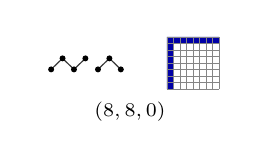
\begin{tikzpicture}[x=1mm,y=1mm,baseline=0mm]
\path[use as bounding box] (0,-1) rectangle (27,11);
\draw[black!78,line width=.43pt] (4.43,7.10)--(5.88,5.70) (4.43,7.10)--(2.98,5.70) (5.88,5.70)--(7.33,7.10);
\fill (4.43,7.10) circle[radius=.38mm];
\fill (5.88,5.70) circle[radius=.38mm];
\fill (2.98,5.70) circle[radius=.38mm];
\fill (7.33,7.10) circle[radius=.38mm];
\draw[black!78,line width=.43pt] (10.38,7.10)--(8.93,5.70) (10.38,7.10)--(11.83,5.70);
\fill (10.38,7.10) circle[radius=.38mm];
\fill (8.93,5.70) circle[radius=.38mm];
\fill (11.83,5.70) circle[radius=.38mm];
\begin{scope}[shift={(17.680,3.180)},x=0.83mm,y=0.83mm]
\fill[blue!65!black] (0,0) rectangle (1,8) (0,7) rectangle (8,8);
\draw[black!48,line width=.16pt] (0,0)--(0,8) (1,0)--(1,8) (2,0)--(2,8) (3,0)--(3,8) (4,0)--(4,8) (5,0)--(5,8) (6,0)--(6,8) (7,0)--(7,8) (8,0)--(8,8) (0,0)--(8,0) (0,1)--(8,1) (0,2)--(8,2) (0,3)--(8,3) (0,4)--(8,4) (0,5)--(8,5) (0,6)--(8,6) (0,7)--(8,7) (0,8)--(8,8);
\end{scope}
\node[font=\scriptsize,inner sep=0pt] at (13,.35) {$(8,8,0)$};
\end{tikzpicture} \\[.5mm]
\end{tabular}
\caption{Order-23 templates with 5 unmarked edges, part 1 of 4.}
\label{fig:nine-chain-3}
\end{figure}

\begin{figure}[!htbp]
\centering
\begin{tabular}{@{}c@{\hspace{2.5mm}}c@{\hspace{2.5mm}}c@{\hspace{2.5mm}}c@{}}
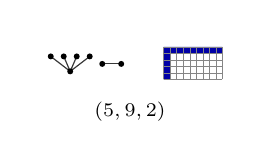
\begin{tikzpicture}[x=1mm,y=1mm,baseline=0mm]
\path[use as bounding box] (0,-1) rectangle (27,11);
\draw[black!78,line width=.43pt] (5.40,5.45)--(2.93,7.35) (5.40,5.45)--(4.58,7.35) (5.40,5.45)--(6.23,7.35) (5.40,5.45)--(7.88,7.35);
\fill (5.40,5.45) circle[radius=.38mm];
\fill (2.93,7.35) circle[radius=.38mm];
\fill (4.58,7.35) circle[radius=.38mm];
\fill (6.23,7.35) circle[radius=.38mm];
\fill (7.88,7.35) circle[radius=.38mm];
\draw[black!78,line width=.43pt] (9.47,6.40)--(11.88,6.40);
\fill (9.47,6.40) circle[radius=.38mm];
\fill (11.88,6.40) circle[radius=.38mm];
\begin{scope}[shift={(17.265,4.425)},x=0.83mm,y=0.83mm]
\fill[blue!65!black] (0,0) rectangle (1,5) (0,4) rectangle (9,5);
\draw[black!48,line width=.16pt] (0,0)--(0,5) (1,0)--(1,5) (2,0)--(2,5) (3,0)--(3,5) (4,0)--(4,5) (5,0)--(5,5) (6,0)--(6,5) (7,0)--(7,5) (8,0)--(8,5) (9,0)--(9,5) (0,0)--(9,0) (0,1)--(9,1) (0,2)--(9,2) (0,3)--(9,3) (0,4)--(9,4) (0,5)--(9,5);
\end{scope}
\node[font=\scriptsize,inner sep=0pt] at (13,.35) {$(5,9,2)$};
\end{tikzpicture} &
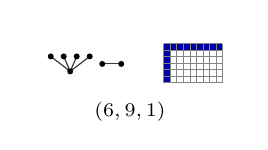
\begin{tikzpicture}[x=1mm,y=1mm,baseline=0mm]
\path[use as bounding box] (0,-1) rectangle (27,11);
\draw[black!78,line width=.43pt] (5.40,5.45)--(2.93,7.35) (5.40,5.45)--(4.58,7.35) (5.40,5.45)--(6.23,7.35) (5.40,5.45)--(7.88,7.35);
\fill (5.40,5.45) circle[radius=.38mm];
\fill (2.93,7.35) circle[radius=.38mm];
\fill (4.58,7.35) circle[radius=.38mm];
\fill (6.23,7.35) circle[radius=.38mm];
\fill (7.88,7.35) circle[radius=.38mm];
\draw[black!78,line width=.43pt] (9.47,6.40)--(11.88,6.40);
\fill (9.47,6.40) circle[radius=.38mm];
\fill (11.88,6.40) circle[radius=.38mm];
\begin{scope}[shift={(17.265,4.010)},x=0.83mm,y=0.83mm]
\fill[blue!65!black] (0,0) rectangle (1,6) (0,5) rectangle (9,6);
\draw[black!48,line width=.16pt] (0,0)--(0,6) (1,0)--(1,6) (2,0)--(2,6) (3,0)--(3,6) (4,0)--(4,6) (5,0)--(5,6) (6,0)--(6,6) (7,0)--(7,6) (8,0)--(8,6) (9,0)--(9,6) (0,0)--(9,0) (0,1)--(9,1) (0,2)--(9,2) (0,3)--(9,3) (0,4)--(9,4) (0,5)--(9,5) (0,6)--(9,6);
\end{scope}
\node[font=\scriptsize,inner sep=0pt] at (13,.35) {$(6,9,1)$};
\end{tikzpicture} &
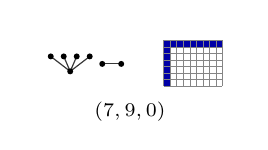
\begin{tikzpicture}[x=1mm,y=1mm,baseline=0mm]
\path[use as bounding box] (0,-1) rectangle (27,11);
\draw[black!78,line width=.43pt] (5.40,5.45)--(2.93,7.35) (5.40,5.45)--(4.58,7.35) (5.40,5.45)--(6.23,7.35) (5.40,5.45)--(7.88,7.35);
\fill (5.40,5.45) circle[radius=.38mm];
\fill (2.93,7.35) circle[radius=.38mm];
\fill (4.58,7.35) circle[radius=.38mm];
\fill (6.23,7.35) circle[radius=.38mm];
\fill (7.88,7.35) circle[radius=.38mm];
\draw[black!78,line width=.43pt] (9.47,6.40)--(11.88,6.40);
\fill (9.47,6.40) circle[radius=.38mm];
\fill (11.88,6.40) circle[radius=.38mm];
\begin{scope}[shift={(17.265,3.595)},x=0.83mm,y=0.83mm]
\fill[blue!65!black] (0,0) rectangle (1,7) (0,6) rectangle (9,7);
\draw[black!48,line width=.16pt] (0,0)--(0,7) (1,0)--(1,7) (2,0)--(2,7) (3,0)--(3,7) (4,0)--(4,7) (5,0)--(5,7) (6,0)--(6,7) (7,0)--(7,7) (8,0)--(8,7) (9,0)--(9,7) (0,0)--(9,0) (0,1)--(9,1) (0,2)--(9,2) (0,3)--(9,3) (0,4)--(9,4) (0,5)--(9,5) (0,6)--(9,6) (0,7)--(9,7);
\end{scope}
\node[font=\scriptsize,inner sep=0pt] at (13,.35) {$(7,9,0)$};
\end{tikzpicture} &
\begin{tikzpicture}[x=1mm,y=1mm,baseline=0mm]
\path[use as bounding box] (0,-1) rectangle (27,11);
\draw[black!78,line width=.43pt] (5.40,5.45)--(2.93,7.35) (5.40,5.45)--(4.58,7.35) (5.40,5.45)--(6.23,7.35) (5.40,5.45)--(7.88,7.35);
\fill (5.40,5.45) circle[radius=.38mm];
\fill (2.93,7.35) circle[radius=.38mm];
\fill (4.58,7.35) circle[radius=.38mm];
\fill (6.23,7.35) circle[radius=.38mm];
\fill (7.88,7.35) circle[radius=.38mm];
\draw[black!78,line width=.43pt] (9.47,6.40)--(11.88,6.40);
\fill (9.47,6.40) circle[radius=.38mm];
\fill (11.88,6.40) circle[radius=.38mm];
\begin{scope}[shift={(17.680,3.180)},x=0.83mm,y=0.83mm]
\fill[blue!65!black] (0,0) rectangle (1,8) (0,7) rectangle (8,8);
\draw[black!48,line width=.16pt] (0,0)--(0,8) (1,0)--(1,8) (2,0)--(2,8) (3,0)--(3,8) (4,0)--(4,8) (5,0)--(5,8) (6,0)--(6,8) (7,0)--(7,8) (8,0)--(8,8) (0,0)--(8,0) (0,1)--(8,1) (0,2)--(8,2) (0,3)--(8,3) (0,4)--(8,4) (0,5)--(8,5) (0,6)--(8,6) (0,7)--(8,7) (0,8)--(8,8);
\end{scope}
\node[font=\scriptsize,inner sep=0pt] at (13,.35) {$(8,8,0)$};
\end{tikzpicture} \\[.5mm]
\begin{tikzpicture}[x=1mm,y=1mm,baseline=0mm]
\path[use as bounding box] (0,-1) rectangle (27,11);
\draw[black!78,line width=.43pt] (5.40,4.50)--(3.75,6.40) (5.40,4.50)--(5.40,6.40) (5.40,4.50)--(7.05,6.40) (3.75,6.40)--(3.75,8.30);
\fill (5.40,4.50) circle[radius=.38mm];
\fill (3.75,6.40) circle[radius=.38mm];
\fill (5.40,6.40) circle[radius=.38mm];
\fill (7.05,6.40) circle[radius=.38mm];
\fill (3.75,8.30) circle[radius=.38mm];
\draw[black!78,line width=.43pt] (8.65,6.40)--(11.05,6.40);
\fill (8.65,6.40) circle[radius=.38mm];
\fill (11.05,6.40) circle[radius=.38mm];
\begin{scope}[shift={(17.265,4.425)},x=0.83mm,y=0.83mm]
\fill[blue!65!black] (0,0) rectangle (1,5) (0,4) rectangle (9,5);
\draw[black!48,line width=.16pt] (0,0)--(0,5) (1,0)--(1,5) (2,0)--(2,5) (3,0)--(3,5) (4,0)--(4,5) (5,0)--(5,5) (6,0)--(6,5) (7,0)--(7,5) (8,0)--(8,5) (9,0)--(9,5) (0,0)--(9,0) (0,1)--(9,1) (0,2)--(9,2) (0,3)--(9,3) (0,4)--(9,4) (0,5)--(9,5);
\end{scope}
\node[font=\scriptsize,inner sep=0pt] at (13,.35) {$(5,9,2)$};
\end{tikzpicture} &
\begin{tikzpicture}[x=1mm,y=1mm,baseline=0mm]
\path[use as bounding box] (0,-1) rectangle (27,11);
\draw[black!78,line width=.43pt] (5.40,4.50)--(3.75,6.40) (5.40,4.50)--(5.40,6.40) (5.40,4.50)--(7.05,6.40) (3.75,6.40)--(3.75,8.30);
\fill (5.40,4.50) circle[radius=.38mm];
\fill (3.75,6.40) circle[radius=.38mm];
\fill (5.40,6.40) circle[radius=.38mm];
\fill (7.05,6.40) circle[radius=.38mm];
\fill (3.75,8.30) circle[radius=.38mm];
\draw[black!78,line width=.43pt] (8.65,6.40)--(11.05,6.40);
\fill (8.65,6.40) circle[radius=.38mm];
\fill (11.05,6.40) circle[radius=.38mm];
\begin{scope}[shift={(17.265,4.010)},x=0.83mm,y=0.83mm]
\fill[blue!65!black] (0,0) rectangle (1,6) (0,5) rectangle (9,6);
\draw[black!48,line width=.16pt] (0,0)--(0,6) (1,0)--(1,6) (2,0)--(2,6) (3,0)--(3,6) (4,0)--(4,6) (5,0)--(5,6) (6,0)--(6,6) (7,0)--(7,6) (8,0)--(8,6) (9,0)--(9,6) (0,0)--(9,0) (0,1)--(9,1) (0,2)--(9,2) (0,3)--(9,3) (0,4)--(9,4) (0,5)--(9,5) (0,6)--(9,6);
\end{scope}
\node[font=\scriptsize,inner sep=0pt] at (13,.35) {$(6,9,1)$};
\end{tikzpicture} &
\begin{tikzpicture}[x=1mm,y=1mm,baseline=0mm]
\path[use as bounding box] (0,-1) rectangle (27,11);
\draw[black!78,line width=.43pt] (5.40,4.50)--(3.75,6.40) (5.40,4.50)--(5.40,6.40) (5.40,4.50)--(7.05,6.40) (3.75,6.40)--(3.75,8.30);
\fill (5.40,4.50) circle[radius=.38mm];
\fill (3.75,6.40) circle[radius=.38mm];
\fill (5.40,6.40) circle[radius=.38mm];
\fill (7.05,6.40) circle[radius=.38mm];
\fill (3.75,8.30) circle[radius=.38mm];
\draw[black!78,line width=.43pt] (8.65,6.40)--(11.05,6.40);
\fill (8.65,6.40) circle[radius=.38mm];
\fill (11.05,6.40) circle[radius=.38mm];
\begin{scope}[shift={(17.265,3.595)},x=0.83mm,y=0.83mm]
\fill[blue!65!black] (0,0) rectangle (1,7) (0,6) rectangle (9,7);
\draw[black!48,line width=.16pt] (0,0)--(0,7) (1,0)--(1,7) (2,0)--(2,7) (3,0)--(3,7) (4,0)--(4,7) (5,0)--(5,7) (6,0)--(6,7) (7,0)--(7,7) (8,0)--(8,7) (9,0)--(9,7) (0,0)--(9,0) (0,1)--(9,1) (0,2)--(9,2) (0,3)--(9,3) (0,4)--(9,4) (0,5)--(9,5) (0,6)--(9,6) (0,7)--(9,7);
\end{scope}
\node[font=\scriptsize,inner sep=0pt] at (13,.35) {$(7,9,0)$};
\end{tikzpicture} &
\begin{tikzpicture}[x=1mm,y=1mm,baseline=0mm]
\path[use as bounding box] (0,-1) rectangle (27,11);
\draw[black!78,line width=.43pt] (5.40,4.50)--(3.75,6.40) (5.40,4.50)--(5.40,6.40) (5.40,4.50)--(7.05,6.40) (3.75,6.40)--(3.75,8.30);
\fill (5.40,4.50) circle[radius=.38mm];
\fill (3.75,6.40) circle[radius=.38mm];
\fill (5.40,6.40) circle[radius=.38mm];
\fill (7.05,6.40) circle[radius=.38mm];
\fill (3.75,8.30) circle[radius=.38mm];
\draw[black!78,line width=.43pt] (8.65,6.40)--(11.05,6.40);
\fill (8.65,6.40) circle[radius=.38mm];
\fill (11.05,6.40) circle[radius=.38mm];
\begin{scope}[shift={(17.680,3.180)},x=0.83mm,y=0.83mm]
\fill[blue!65!black] (0,0) rectangle (1,8) (0,7) rectangle (8,8);
\draw[black!48,line width=.16pt] (0,0)--(0,8) (1,0)--(1,8) (2,0)--(2,8) (3,0)--(3,8) (4,0)--(4,8) (5,0)--(5,8) (6,0)--(6,8) (7,0)--(7,8) (8,0)--(8,8) (0,0)--(8,0) (0,1)--(8,1) (0,2)--(8,2) (0,3)--(8,3) (0,4)--(8,4) (0,5)--(8,5) (0,6)--(8,6) (0,7)--(8,7) (0,8)--(8,8);
\end{scope}
\node[font=\scriptsize,inner sep=0pt] at (13,.35) {$(8,8,0)$};
\end{tikzpicture} \\[.5mm]
\begin{tikzpicture}[x=1mm,y=1mm,baseline=0mm]
\path[use as bounding box] (0,-1) rectangle (27,11);
\draw[black!78,line width=.43pt] (5.40,5.70)--(3.95,7.10) (5.40,5.70)--(6.85,7.10) (3.95,7.10)--(2.50,5.70) (6.85,7.10)--(8.30,5.70);
\fill (5.40,5.70) circle[radius=.38mm];
\fill (3.95,7.10) circle[radius=.38mm];
\fill (6.85,7.10) circle[radius=.38mm];
\fill (2.50,5.70) circle[radius=.38mm];
\fill (8.30,5.70) circle[radius=.38mm];
\draw[black!78,line width=.43pt] (9.90,6.40)--(12.30,6.40);
\fill (9.90,6.40) circle[radius=.38mm];
\fill (12.30,6.40) circle[radius=.38mm];
\begin{scope}[shift={(17.265,4.425)},x=0.83mm,y=0.83mm]
\fill[blue!65!black] (0,0) rectangle (1,5) (0,4) rectangle (9,5);
\draw[black!48,line width=.16pt] (0,0)--(0,5) (1,0)--(1,5) (2,0)--(2,5) (3,0)--(3,5) (4,0)--(4,5) (5,0)--(5,5) (6,0)--(6,5) (7,0)--(7,5) (8,0)--(8,5) (9,0)--(9,5) (0,0)--(9,0) (0,1)--(9,1) (0,2)--(9,2) (0,3)--(9,3) (0,4)--(9,4) (0,5)--(9,5);
\end{scope}
\node[font=\scriptsize,inner sep=0pt] at (13,.35) {$(5,9,2)$};
\end{tikzpicture} &
\begin{tikzpicture}[x=1mm,y=1mm,baseline=0mm]
\path[use as bounding box] (0,-1) rectangle (27,11);
\draw[black!78,line width=.43pt] (5.40,5.70)--(3.95,7.10) (5.40,5.70)--(6.85,7.10) (3.95,7.10)--(2.50,5.70) (6.85,7.10)--(8.30,5.70);
\fill (5.40,5.70) circle[radius=.38mm];
\fill (3.95,7.10) circle[radius=.38mm];
\fill (6.85,7.10) circle[radius=.38mm];
\fill (2.50,5.70) circle[radius=.38mm];
\fill (8.30,5.70) circle[radius=.38mm];
\draw[black!78,line width=.43pt] (9.90,6.40)--(12.30,6.40);
\fill (9.90,6.40) circle[radius=.38mm];
\fill (12.30,6.40) circle[radius=.38mm];
\begin{scope}[shift={(17.265,4.010)},x=0.83mm,y=0.83mm]
\fill[blue!65!black] (0,0) rectangle (1,6) (0,5) rectangle (9,6);
\draw[black!48,line width=.16pt] (0,0)--(0,6) (1,0)--(1,6) (2,0)--(2,6) (3,0)--(3,6) (4,0)--(4,6) (5,0)--(5,6) (6,0)--(6,6) (7,0)--(7,6) (8,0)--(8,6) (9,0)--(9,6) (0,0)--(9,0) (0,1)--(9,1) (0,2)--(9,2) (0,3)--(9,3) (0,4)--(9,4) (0,5)--(9,5) (0,6)--(9,6);
\end{scope}
\node[font=\scriptsize,inner sep=0pt] at (13,.35) {$(6,9,1)$};
\end{tikzpicture} &
\begin{tikzpicture}[x=1mm,y=1mm,baseline=0mm]
\path[use as bounding box] (0,-1) rectangle (27,11);
\draw[black!78,line width=.43pt] (5.40,5.70)--(3.95,7.10) (5.40,5.70)--(6.85,7.10) (3.95,7.10)--(2.50,5.70) (6.85,7.10)--(8.30,5.70);
\fill (5.40,5.70) circle[radius=.38mm];
\fill (3.95,7.10) circle[radius=.38mm];
\fill (6.85,7.10) circle[radius=.38mm];
\fill (2.50,5.70) circle[radius=.38mm];
\fill (8.30,5.70) circle[radius=.38mm];
\draw[black!78,line width=.43pt] (9.90,6.40)--(12.30,6.40);
\fill (9.90,6.40) circle[radius=.38mm];
\fill (12.30,6.40) circle[radius=.38mm];
\begin{scope}[shift={(17.265,3.595)},x=0.83mm,y=0.83mm]
\fill[blue!65!black] (0,0) rectangle (1,7) (0,6) rectangle (9,7);
\draw[black!48,line width=.16pt] (0,0)--(0,7) (1,0)--(1,7) (2,0)--(2,7) (3,0)--(3,7) (4,0)--(4,7) (5,0)--(5,7) (6,0)--(6,7) (7,0)--(7,7) (8,0)--(8,7) (9,0)--(9,7) (0,0)--(9,0) (0,1)--(9,1) (0,2)--(9,2) (0,3)--(9,3) (0,4)--(9,4) (0,5)--(9,5) (0,6)--(9,6) (0,7)--(9,7);
\end{scope}
\node[font=\scriptsize,inner sep=0pt] at (13,.35) {$(7,9,0)$};
\end{tikzpicture} &
\begin{tikzpicture}[x=1mm,y=1mm,baseline=0mm]
\path[use as bounding box] (0,-1) rectangle (27,11);
\draw[black!78,line width=.43pt] (5.40,5.70)--(3.95,7.10) (5.40,5.70)--(6.85,7.10) (3.95,7.10)--(2.50,5.70) (6.85,7.10)--(8.30,5.70);
\fill (5.40,5.70) circle[radius=.38mm];
\fill (3.95,7.10) circle[radius=.38mm];
\fill (6.85,7.10) circle[radius=.38mm];
\fill (2.50,5.70) circle[radius=.38mm];
\fill (8.30,5.70) circle[radius=.38mm];
\draw[black!78,line width=.43pt] (9.90,6.40)--(12.30,6.40);
\fill (9.90,6.40) circle[radius=.38mm];
\fill (12.30,6.40) circle[radius=.38mm];
\begin{scope}[shift={(17.680,3.180)},x=0.83mm,y=0.83mm]
\fill[blue!65!black] (0,0) rectangle (1,8) (0,7) rectangle (8,8);
\draw[black!48,line width=.16pt] (0,0)--(0,8) (1,0)--(1,8) (2,0)--(2,8) (3,0)--(3,8) (4,0)--(4,8) (5,0)--(5,8) (6,0)--(6,8) (7,0)--(7,8) (8,0)--(8,8) (0,0)--(8,0) (0,1)--(8,1) (0,2)--(8,2) (0,3)--(8,3) (0,4)--(8,4) (0,5)--(8,5) (0,6)--(8,6) (0,7)--(8,7) (0,8)--(8,8);
\end{scope}
\node[font=\scriptsize,inner sep=0pt] at (13,.35) {$(8,8,0)$};
\end{tikzpicture} \\[.5mm]
\begin{tikzpicture}[x=1mm,y=1mm,baseline=0mm]
\path[use as bounding box] (0,-1) rectangle (27,11);
\draw[black!78,line width=.43pt] (3.40,7.83)--(1.75,4.98) (3.40,7.83)--(5.05,4.97) (1.75,4.98)--(5.05,4.97);
\fill (3.40,7.83) circle[radius=.38mm];
\fill (1.75,4.98) circle[radius=.38mm];
\fill (5.05,4.97) circle[radius=.38mm];
\draw[black!78,line width=.43pt] (6.65,6.40)--(9.05,6.40);
\fill (6.65,6.40) circle[radius=.38mm];
\fill (9.05,6.40) circle[radius=.38mm];
\draw[black!78,line width=.43pt] (10.65,6.40)--(13.05,6.40);
\fill (10.65,6.40) circle[radius=.38mm];
\fill (13.05,6.40) circle[radius=.38mm];
\begin{scope}[shift={(17.265,4.425)},x=0.83mm,y=0.83mm]
\fill[blue!65!black] (0,0) rectangle (1,5) (0,4) rectangle (9,5);
\draw[black!48,line width=.16pt] (0,0)--(0,5) (1,0)--(1,5) (2,0)--(2,5) (3,0)--(3,5) (4,0)--(4,5) (5,0)--(5,5) (6,0)--(6,5) (7,0)--(7,5) (8,0)--(8,5) (9,0)--(9,5) (0,0)--(9,0) (0,1)--(9,1) (0,2)--(9,2) (0,3)--(9,3) (0,4)--(9,4) (0,5)--(9,5);
\end{scope}
\node[font=\scriptsize,inner sep=0pt] at (13,.35) {$(5,9,2)$};
\end{tikzpicture} &
\begin{tikzpicture}[x=1mm,y=1mm,baseline=0mm]
\path[use as bounding box] (0,-1) rectangle (27,11);
\draw[black!78,line width=.43pt] (3.40,7.83)--(1.75,4.98) (3.40,7.83)--(5.05,4.97) (1.75,4.98)--(5.05,4.97);
\fill (3.40,7.83) circle[radius=.38mm];
\fill (1.75,4.98) circle[radius=.38mm];
\fill (5.05,4.97) circle[radius=.38mm];
\draw[black!78,line width=.43pt] (6.65,6.40)--(9.05,6.40);
\fill (6.65,6.40) circle[radius=.38mm];
\fill (9.05,6.40) circle[radius=.38mm];
\draw[black!78,line width=.43pt] (10.65,6.40)--(13.05,6.40);
\fill (10.65,6.40) circle[radius=.38mm];
\fill (13.05,6.40) circle[radius=.38mm];
\begin{scope}[shift={(17.265,4.010)},x=0.83mm,y=0.83mm]
\fill[blue!65!black] (0,0) rectangle (1,6) (0,5) rectangle (9,6);
\draw[black!48,line width=.16pt] (0,0)--(0,6) (1,0)--(1,6) (2,0)--(2,6) (3,0)--(3,6) (4,0)--(4,6) (5,0)--(5,6) (6,0)--(6,6) (7,0)--(7,6) (8,0)--(8,6) (9,0)--(9,6) (0,0)--(9,0) (0,1)--(9,1) (0,2)--(9,2) (0,3)--(9,3) (0,4)--(9,4) (0,5)--(9,5) (0,6)--(9,6);
\end{scope}
\node[font=\scriptsize,inner sep=0pt] at (13,.35) {$(6,9,1)$};
\end{tikzpicture} &
\begin{tikzpicture}[x=1mm,y=1mm,baseline=0mm]
\path[use as bounding box] (0,-1) rectangle (27,11);
\draw[black!78,line width=.43pt] (3.40,7.83)--(1.75,4.98) (3.40,7.83)--(5.05,4.97) (1.75,4.98)--(5.05,4.97);
\fill (3.40,7.83) circle[radius=.38mm];
\fill (1.75,4.98) circle[radius=.38mm];
\fill (5.05,4.97) circle[radius=.38mm];
\draw[black!78,line width=.43pt] (6.65,6.40)--(9.05,6.40);
\fill (6.65,6.40) circle[radius=.38mm];
\fill (9.05,6.40) circle[radius=.38mm];
\draw[black!78,line width=.43pt] (10.65,6.40)--(13.05,6.40);
\fill (10.65,6.40) circle[radius=.38mm];
\fill (13.05,6.40) circle[radius=.38mm];
\begin{scope}[shift={(17.265,3.595)},x=0.83mm,y=0.83mm]
\fill[blue!65!black] (0,0) rectangle (1,7) (0,6) rectangle (9,7);
\draw[black!48,line width=.16pt] (0,0)--(0,7) (1,0)--(1,7) (2,0)--(2,7) (3,0)--(3,7) (4,0)--(4,7) (5,0)--(5,7) (6,0)--(6,7) (7,0)--(7,7) (8,0)--(8,7) (9,0)--(9,7) (0,0)--(9,0) (0,1)--(9,1) (0,2)--(9,2) (0,3)--(9,3) (0,4)--(9,4) (0,5)--(9,5) (0,6)--(9,6) (0,7)--(9,7);
\end{scope}
\node[font=\scriptsize,inner sep=0pt] at (13,.35) {$(7,9,0)$};
\end{tikzpicture} &
\begin{tikzpicture}[x=1mm,y=1mm,baseline=0mm]
\path[use as bounding box] (0,-1) rectangle (27,11);
\draw[black!78,line width=.43pt] (3.40,7.83)--(1.75,4.98) (3.40,7.83)--(5.05,4.97) (1.75,4.98)--(5.05,4.97);
\fill (3.40,7.83) circle[radius=.38mm];
\fill (1.75,4.98) circle[radius=.38mm];
\fill (5.05,4.97) circle[radius=.38mm];
\draw[black!78,line width=.43pt] (6.65,6.40)--(9.05,6.40);
\fill (6.65,6.40) circle[radius=.38mm];
\fill (9.05,6.40) circle[radius=.38mm];
\draw[black!78,line width=.43pt] (10.65,6.40)--(13.05,6.40);
\fill (10.65,6.40) circle[radius=.38mm];
\fill (13.05,6.40) circle[radius=.38mm];
\begin{scope}[shift={(17.680,3.180)},x=0.83mm,y=0.83mm]
\fill[blue!65!black] (0,0) rectangle (1,8) (0,7) rectangle (8,8);
\draw[black!48,line width=.16pt] (0,0)--(0,8) (1,0)--(1,8) (2,0)--(2,8) (3,0)--(3,8) (4,0)--(4,8) (5,0)--(5,8) (6,0)--(6,8) (7,0)--(7,8) (8,0)--(8,8) (0,0)--(8,0) (0,1)--(8,1) (0,2)--(8,2) (0,3)--(8,3) (0,4)--(8,4) (0,5)--(8,5) (0,6)--(8,6) (0,7)--(8,7) (0,8)--(8,8);
\end{scope}
\node[font=\scriptsize,inner sep=0pt] at (13,.35) {$(8,8,0)$};
\end{tikzpicture} \\[.5mm]
\begin{tikzpicture}[x=1mm,y=1mm,baseline=0mm]
\path[use as bounding box] (0,-1) rectangle (27,11);
\draw[black!78,line width=.43pt] (3.15,7.10)--(1.70,5.70) (3.15,7.10)--(4.60,5.70);
\fill (3.15,7.10) circle[radius=.38mm];
\fill (1.70,5.70) circle[radius=.38mm];
\fill (4.60,5.70) circle[radius=.38mm];
\draw[black!78,line width=.43pt] (7.65,7.10)--(6.20,5.70) (7.65,7.10)--(9.10,5.70);
\fill (7.65,7.10) circle[radius=.38mm];
\fill (6.20,5.70) circle[radius=.38mm];
\fill (9.10,5.70) circle[radius=.38mm];
\draw[black!78,line width=.43pt] (10.70,6.40)--(13.10,6.40);
\fill (10.70,6.40) circle[radius=.38mm];
\fill (13.10,6.40) circle[radius=.38mm];
\begin{scope}[shift={(17.265,4.840)},x=0.83mm,y=0.83mm]
\fill[blue!65!black] (0,0) rectangle (1,4) (0,3) rectangle (9,4);
\draw[black!48,line width=.16pt] (0,0)--(0,4) (1,0)--(1,4) (2,0)--(2,4) (3,0)--(3,4) (4,0)--(4,4) (5,0)--(5,4) (6,0)--(6,4) (7,0)--(7,4) (8,0)--(8,4) (9,0)--(9,4) (0,0)--(9,0) (0,1)--(9,1) (0,2)--(9,2) (0,3)--(9,3) (0,4)--(9,4);
\end{scope}
\node[font=\scriptsize,inner sep=0pt] at (13,.35) {$(4,9,2)$};
\end{tikzpicture} &
\begin{tikzpicture}[x=1mm,y=1mm,baseline=0mm]
\path[use as bounding box] (0,-1) rectangle (27,11);
\draw[black!78,line width=.43pt] (3.15,7.10)--(1.70,5.70) (3.15,7.10)--(4.60,5.70);
\fill (3.15,7.10) circle[radius=.38mm];
\fill (1.70,5.70) circle[radius=.38mm];
\fill (4.60,5.70) circle[radius=.38mm];
\draw[black!78,line width=.43pt] (7.65,7.10)--(6.20,5.70) (7.65,7.10)--(9.10,5.70);
\fill (7.65,7.10) circle[radius=.38mm];
\fill (6.20,5.70) circle[radius=.38mm];
\fill (9.10,5.70) circle[radius=.38mm];
\draw[black!78,line width=.43pt] (10.70,6.40)--(13.10,6.40);
\fill (10.70,6.40) circle[radius=.38mm];
\fill (13.10,6.40) circle[radius=.38mm];
\begin{scope}[shift={(17.680,4.425)},x=0.83mm,y=0.83mm]
\fill[blue!65!black] (0,0) rectangle (1,5) (0,4) rectangle (8,5);
\draw[black!48,line width=.16pt] (0,0)--(0,5) (1,0)--(1,5) (2,0)--(2,5) (3,0)--(3,5) (4,0)--(4,5) (5,0)--(5,5) (6,0)--(6,5) (7,0)--(7,5) (8,0)--(8,5) (0,0)--(8,0) (0,1)--(8,1) (0,2)--(8,2) (0,3)--(8,3) (0,4)--(8,4) (0,5)--(8,5);
\end{scope}
\node[font=\scriptsize,inner sep=0pt] at (13,.35) {$(5,8,2)$};
\end{tikzpicture} &
\begin{tikzpicture}[x=1mm,y=1mm,baseline=0mm]
\path[use as bounding box] (0,-1) rectangle (27,11);
\draw[black!78,line width=.43pt] (3.15,7.10)--(1.70,5.70) (3.15,7.10)--(4.60,5.70);
\fill (3.15,7.10) circle[radius=.38mm];
\fill (1.70,5.70) circle[radius=.38mm];
\fill (4.60,5.70) circle[radius=.38mm];
\draw[black!78,line width=.43pt] (7.65,7.10)--(6.20,5.70) (7.65,7.10)--(9.10,5.70);
\fill (7.65,7.10) circle[radius=.38mm];
\fill (6.20,5.70) circle[radius=.38mm];
\fill (9.10,5.70) circle[radius=.38mm];
\draw[black!78,line width=.43pt] (10.70,6.40)--(13.10,6.40);
\fill (10.70,6.40) circle[radius=.38mm];
\fill (13.10,6.40) circle[radius=.38mm];
\begin{scope}[shift={(17.265,4.425)},x=0.83mm,y=0.83mm]
\fill[blue!65!black] (0,0) rectangle (1,5) (0,4) rectangle (9,5);
\draw[black!48,line width=.16pt] (0,0)--(0,5) (1,0)--(1,5) (2,0)--(2,5) (3,0)--(3,5) (4,0)--(4,5) (5,0)--(5,5) (6,0)--(6,5) (7,0)--(7,5) (8,0)--(8,5) (9,0)--(9,5) (0,0)--(9,0) (0,1)--(9,1) (0,2)--(9,2) (0,3)--(9,3) (0,4)--(9,4) (0,5)--(9,5);
\end{scope}
\node[font=\scriptsize,inner sep=0pt] at (13,.35) {$(5,9,1)$};
\end{tikzpicture} &
\begin{tikzpicture}[x=1mm,y=1mm,baseline=0mm]
\path[use as bounding box] (0,-1) rectangle (27,11);
\draw[black!78,line width=.43pt] (3.15,7.10)--(1.70,5.70) (3.15,7.10)--(4.60,5.70);
\fill (3.15,7.10) circle[radius=.38mm];
\fill (1.70,5.70) circle[radius=.38mm];
\fill (4.60,5.70) circle[radius=.38mm];
\draw[black!78,line width=.43pt] (7.65,7.10)--(6.20,5.70) (7.65,7.10)--(9.10,5.70);
\fill (7.65,7.10) circle[radius=.38mm];
\fill (6.20,5.70) circle[radius=.38mm];
\fill (9.10,5.70) circle[radius=.38mm];
\draw[black!78,line width=.43pt] (10.70,6.40)--(13.10,6.40);
\fill (10.70,6.40) circle[radius=.38mm];
\fill (13.10,6.40) circle[radius=.38mm];
\begin{scope}[shift={(17.680,4.010)},x=0.83mm,y=0.83mm]
\fill[blue!65!black] (0,0) rectangle (1,6) (0,5) rectangle (8,6);
\draw[black!48,line width=.16pt] (0,0)--(0,6) (1,0)--(1,6) (2,0)--(2,6) (3,0)--(3,6) (4,0)--(4,6) (5,0)--(5,6) (6,0)--(6,6) (7,0)--(7,6) (8,0)--(8,6) (0,0)--(8,0) (0,1)--(8,1) (0,2)--(8,2) (0,3)--(8,3) (0,4)--(8,4) (0,5)--(8,5) (0,6)--(8,6);
\end{scope}
\node[font=\scriptsize,inner sep=0pt] at (13,.35) {$(6,8,1)$};
\end{tikzpicture} \\[.5mm]
\begin{tikzpicture}[x=1mm,y=1mm,baseline=0mm]
\path[use as bounding box] (0,-1) rectangle (27,11);
\draw[black!78,line width=.43pt] (3.15,7.10)--(1.70,5.70) (3.15,7.10)--(4.60,5.70);
\fill (3.15,7.10) circle[radius=.38mm];
\fill (1.70,5.70) circle[radius=.38mm];
\fill (4.60,5.70) circle[radius=.38mm];
\draw[black!78,line width=.43pt] (7.65,7.10)--(6.20,5.70) (7.65,7.10)--(9.10,5.70);
\fill (7.65,7.10) circle[radius=.38mm];
\fill (6.20,5.70) circle[radius=.38mm];
\fill (9.10,5.70) circle[radius=.38mm];
\draw[black!78,line width=.43pt] (10.70,6.40)--(13.10,6.40);
\fill (10.70,6.40) circle[radius=.38mm];
\fill (13.10,6.40) circle[radius=.38mm];
\begin{scope}[shift={(17.265,4.010)},x=0.83mm,y=0.83mm]
\fill[blue!65!black] (0,0) rectangle (1,6) (0,5) rectangle (9,6);
\draw[black!48,line width=.16pt] (0,0)--(0,6) (1,0)--(1,6) (2,0)--(2,6) (3,0)--(3,6) (4,0)--(4,6) (5,0)--(5,6) (6,0)--(6,6) (7,0)--(7,6) (8,0)--(8,6) (9,0)--(9,6) (0,0)--(9,0) (0,1)--(9,1) (0,2)--(9,2) (0,3)--(9,3) (0,4)--(9,4) (0,5)--(9,5) (0,6)--(9,6);
\end{scope}
\node[font=\scriptsize,inner sep=0pt] at (13,.35) {$(6,9,0)^{*}$};
\end{tikzpicture} &
\begin{tikzpicture}[x=1mm,y=1mm,baseline=0mm]
\path[use as bounding box] (0,-1) rectangle (27,11);
\draw[black!78,line width=.43pt] (3.15,7.10)--(1.70,5.70) (3.15,7.10)--(4.60,5.70);
\fill (3.15,7.10) circle[radius=.38mm];
\fill (1.70,5.70) circle[radius=.38mm];
\fill (4.60,5.70) circle[radius=.38mm];
\draw[black!78,line width=.43pt] (7.65,7.10)--(6.20,5.70) (7.65,7.10)--(9.10,5.70);
\fill (7.65,7.10) circle[radius=.38mm];
\fill (6.20,5.70) circle[radius=.38mm];
\fill (9.10,5.70) circle[radius=.38mm];
\draw[black!78,line width=.43pt] (10.70,6.40)--(13.10,6.40);
\fill (10.70,6.40) circle[radius=.38mm];
\fill (13.10,6.40) circle[radius=.38mm];
\begin{scope}[shift={(18.095,3.595)},x=0.83mm,y=0.83mm]
\fill[blue!65!black] (0,0) rectangle (1,7) (0,6) rectangle (7,7);
\draw[black!48,line width=.16pt] (0,0)--(0,7) (1,0)--(1,7) (2,0)--(2,7) (3,0)--(3,7) (4,0)--(4,7) (5,0)--(5,7) (6,0)--(6,7) (7,0)--(7,7) (0,0)--(7,0) (0,1)--(7,1) (0,2)--(7,2) (0,3)--(7,3) (0,4)--(7,4) (0,5)--(7,5) (0,6)--(7,6) (0,7)--(7,7);
\end{scope}
\node[font=\scriptsize,inner sep=0pt] at (13,.35) {$(7,7,1)$};
\end{tikzpicture} \\[.5mm]
\end{tabular}
\caption{Order-23 templates with 5 unmarked edges, part 2 of 4. Starred templates also occur in the triangle-free list.}
\label{fig:nine-chain-4}
\end{figure}

\begin{figure}[!htbp]
\centering
\begin{tabular}{@{}c@{\hspace{2.5mm}}c@{\hspace{2.5mm}}c@{\hspace{2.5mm}}c@{}}
\begin{tikzpicture}[x=1mm,y=1mm,baseline=0mm]
\path[use as bounding box] (0,-1) rectangle (27,11);
\draw[black!78,line width=.43pt] (3.15,7.10)--(1.70,5.70) (3.15,7.10)--(4.60,5.70);
\fill (3.15,7.10) circle[radius=.38mm];
\fill (1.70,5.70) circle[radius=.38mm];
\fill (4.60,5.70) circle[radius=.38mm];
\draw[black!78,line width=.43pt] (7.65,7.10)--(6.20,5.70) (7.65,7.10)--(9.10,5.70);
\fill (7.65,7.10) circle[radius=.38mm];
\fill (6.20,5.70) circle[radius=.38mm];
\fill (9.10,5.70) circle[radius=.38mm];
\draw[black!78,line width=.43pt] (10.70,6.40)--(13.10,6.40);
\fill (10.70,6.40) circle[radius=.38mm];
\fill (13.10,6.40) circle[radius=.38mm];
\begin{scope}[shift={(17.680,3.595)},x=0.83mm,y=0.83mm]
\fill[blue!65!black] (0,0) rectangle (1,7) (0,6) rectangle (8,7);
\draw[black!48,line width=.16pt] (0,0)--(0,7) (1,0)--(1,7) (2,0)--(2,7) (3,0)--(3,7) (4,0)--(4,7) (5,0)--(5,7) (6,0)--(6,7) (7,0)--(7,7) (8,0)--(8,7) (0,0)--(8,0) (0,1)--(8,1) (0,2)--(8,2) (0,3)--(8,3) (0,4)--(8,4) (0,5)--(8,5) (0,6)--(8,6) (0,7)--(8,7);
\end{scope}
\node[font=\scriptsize,inner sep=0pt] at (13,.35) {$(7,8,0)^{*}$};
\end{tikzpicture} &
\begin{tikzpicture}[x=1mm,y=1mm,baseline=0mm]
\path[use as bounding box] (0,-1) rectangle (27,11);
\draw[black!78,line width=.43pt] (3.40,5.45)--(1.75,7.35) (3.40,5.45)--(3.40,7.35) (3.40,5.45)--(5.05,7.35);
\fill (3.40,5.45) circle[radius=.38mm];
\fill (1.75,7.35) circle[radius=.38mm];
\fill (3.40,7.35) circle[radius=.38mm];
\fill (5.05,7.35) circle[radius=.38mm];
\draw[black!78,line width=.43pt] (6.65,6.40)--(9.05,6.40);
\fill (6.65,6.40) circle[radius=.38mm];
\fill (9.05,6.40) circle[radius=.38mm];
\draw[black!78,line width=.43pt] (10.65,6.40)--(13.05,6.40);
\fill (10.65,6.40) circle[radius=.38mm];
\fill (13.05,6.40) circle[radius=.38mm];
\begin{scope}[shift={(17.265,4.840)},x=0.83mm,y=0.83mm]
\fill[blue!65!black] (0,0) rectangle (1,4) (0,3) rectangle (9,4);
\draw[black!48,line width=.16pt] (0,0)--(0,4) (1,0)--(1,4) (2,0)--(2,4) (3,0)--(3,4) (4,0)--(4,4) (5,0)--(5,4) (6,0)--(6,4) (7,0)--(7,4) (8,0)--(8,4) (9,0)--(9,4) (0,0)--(9,0) (0,1)--(9,1) (0,2)--(9,2) (0,3)--(9,3) (0,4)--(9,4);
\end{scope}
\node[font=\scriptsize,inner sep=0pt] at (13,.35) {$(4,9,2)$};
\end{tikzpicture} &
\begin{tikzpicture}[x=1mm,y=1mm,baseline=0mm]
\path[use as bounding box] (0,-1) rectangle (27,11);
\draw[black!78,line width=.43pt] (3.40,5.45)--(1.75,7.35) (3.40,5.45)--(3.40,7.35) (3.40,5.45)--(5.05,7.35);
\fill (3.40,5.45) circle[radius=.38mm];
\fill (1.75,7.35) circle[radius=.38mm];
\fill (3.40,7.35) circle[radius=.38mm];
\fill (5.05,7.35) circle[radius=.38mm];
\draw[black!78,line width=.43pt] (6.65,6.40)--(9.05,6.40);
\fill (6.65,6.40) circle[radius=.38mm];
\fill (9.05,6.40) circle[radius=.38mm];
\draw[black!78,line width=.43pt] (10.65,6.40)--(13.05,6.40);
\fill (10.65,6.40) circle[radius=.38mm];
\fill (13.05,6.40) circle[radius=.38mm];
\begin{scope}[shift={(17.680,4.425)},x=0.83mm,y=0.83mm]
\fill[blue!65!black] (0,0) rectangle (1,5) (0,4) rectangle (8,5);
\draw[black!48,line width=.16pt] (0,0)--(0,5) (1,0)--(1,5) (2,0)--(2,5) (3,0)--(3,5) (4,0)--(4,5) (5,0)--(5,5) (6,0)--(6,5) (7,0)--(7,5) (8,0)--(8,5) (0,0)--(8,0) (0,1)--(8,1) (0,2)--(8,2) (0,3)--(8,3) (0,4)--(8,4) (0,5)--(8,5);
\end{scope}
\node[font=\scriptsize,inner sep=0pt] at (13,.35) {$(5,8,2)$};
\end{tikzpicture} &
\begin{tikzpicture}[x=1mm,y=1mm,baseline=0mm]
\path[use as bounding box] (0,-1) rectangle (27,11);
\draw[black!78,line width=.43pt] (3.40,5.45)--(1.75,7.35) (3.40,5.45)--(3.40,7.35) (3.40,5.45)--(5.05,7.35);
\fill (3.40,5.45) circle[radius=.38mm];
\fill (1.75,7.35) circle[radius=.38mm];
\fill (3.40,7.35) circle[radius=.38mm];
\fill (5.05,7.35) circle[radius=.38mm];
\draw[black!78,line width=.43pt] (6.65,6.40)--(9.05,6.40);
\fill (6.65,6.40) circle[radius=.38mm];
\fill (9.05,6.40) circle[radius=.38mm];
\draw[black!78,line width=.43pt] (10.65,6.40)--(13.05,6.40);
\fill (10.65,6.40) circle[radius=.38mm];
\fill (13.05,6.40) circle[radius=.38mm];
\begin{scope}[shift={(17.265,4.425)},x=0.83mm,y=0.83mm]
\fill[blue!65!black] (0,0) rectangle (1,5) (0,4) rectangle (9,5);
\draw[black!48,line width=.16pt] (0,0)--(0,5) (1,0)--(1,5) (2,0)--(2,5) (3,0)--(3,5) (4,0)--(4,5) (5,0)--(5,5) (6,0)--(6,5) (7,0)--(7,5) (8,0)--(8,5) (9,0)--(9,5) (0,0)--(9,0) (0,1)--(9,1) (0,2)--(9,2) (0,3)--(9,3) (0,4)--(9,4) (0,5)--(9,5);
\end{scope}
\node[font=\scriptsize,inner sep=0pt] at (13,.35) {$(5,9,1)$};
\end{tikzpicture} \\[.5mm]
\begin{tikzpicture}[x=1mm,y=1mm,baseline=0mm]
\path[use as bounding box] (0,-1) rectangle (27,11);
\draw[black!78,line width=.43pt] (3.40,5.45)--(1.75,7.35) (3.40,5.45)--(3.40,7.35) (3.40,5.45)--(5.05,7.35);
\fill (3.40,5.45) circle[radius=.38mm];
\fill (1.75,7.35) circle[radius=.38mm];
\fill (3.40,7.35) circle[radius=.38mm];
\fill (5.05,7.35) circle[radius=.38mm];
\draw[black!78,line width=.43pt] (6.65,6.40)--(9.05,6.40);
\fill (6.65,6.40) circle[radius=.38mm];
\fill (9.05,6.40) circle[radius=.38mm];
\draw[black!78,line width=.43pt] (10.65,6.40)--(13.05,6.40);
\fill (10.65,6.40) circle[radius=.38mm];
\fill (13.05,6.40) circle[radius=.38mm];
\begin{scope}[shift={(17.680,4.010)},x=0.83mm,y=0.83mm]
\fill[blue!65!black] (0,0) rectangle (1,6) (0,5) rectangle (8,6);
\draw[black!48,line width=.16pt] (0,0)--(0,6) (1,0)--(1,6) (2,0)--(2,6) (3,0)--(3,6) (4,0)--(4,6) (5,0)--(5,6) (6,0)--(6,6) (7,0)--(7,6) (8,0)--(8,6) (0,0)--(8,0) (0,1)--(8,1) (0,2)--(8,2) (0,3)--(8,3) (0,4)--(8,4) (0,5)--(8,5) (0,6)--(8,6);
\end{scope}
\node[font=\scriptsize,inner sep=0pt] at (13,.35) {$(6,8,1)$};
\end{tikzpicture} &
\begin{tikzpicture}[x=1mm,y=1mm,baseline=0mm]
\path[use as bounding box] (0,-1) rectangle (27,11);
\draw[black!78,line width=.43pt] (3.40,5.45)--(1.75,7.35) (3.40,5.45)--(3.40,7.35) (3.40,5.45)--(5.05,7.35);
\fill (3.40,5.45) circle[radius=.38mm];
\fill (1.75,7.35) circle[radius=.38mm];
\fill (3.40,7.35) circle[radius=.38mm];
\fill (5.05,7.35) circle[radius=.38mm];
\draw[black!78,line width=.43pt] (6.65,6.40)--(9.05,6.40);
\fill (6.65,6.40) circle[radius=.38mm];
\fill (9.05,6.40) circle[radius=.38mm];
\draw[black!78,line width=.43pt] (10.65,6.40)--(13.05,6.40);
\fill (10.65,6.40) circle[radius=.38mm];
\fill (13.05,6.40) circle[radius=.38mm];
\begin{scope}[shift={(17.265,4.010)},x=0.83mm,y=0.83mm]
\fill[blue!65!black] (0,0) rectangle (1,6) (0,5) rectangle (9,6);
\draw[black!48,line width=.16pt] (0,0)--(0,6) (1,0)--(1,6) (2,0)--(2,6) (3,0)--(3,6) (4,0)--(4,6) (5,0)--(5,6) (6,0)--(6,6) (7,0)--(7,6) (8,0)--(8,6) (9,0)--(9,6) (0,0)--(9,0) (0,1)--(9,1) (0,2)--(9,2) (0,3)--(9,3) (0,4)--(9,4) (0,5)--(9,5) (0,6)--(9,6);
\end{scope}
\node[font=\scriptsize,inner sep=0pt] at (13,.35) {$(6,9,0)^{*}$};
\end{tikzpicture} &
\begin{tikzpicture}[x=1mm,y=1mm,baseline=0mm]
\path[use as bounding box] (0,-1) rectangle (27,11);
\draw[black!78,line width=.43pt] (3.40,5.45)--(1.75,7.35) (3.40,5.45)--(3.40,7.35) (3.40,5.45)--(5.05,7.35);
\fill (3.40,5.45) circle[radius=.38mm];
\fill (1.75,7.35) circle[radius=.38mm];
\fill (3.40,7.35) circle[radius=.38mm];
\fill (5.05,7.35) circle[radius=.38mm];
\draw[black!78,line width=.43pt] (6.65,6.40)--(9.05,6.40);
\fill (6.65,6.40) circle[radius=.38mm];
\fill (9.05,6.40) circle[radius=.38mm];
\draw[black!78,line width=.43pt] (10.65,6.40)--(13.05,6.40);
\fill (10.65,6.40) circle[radius=.38mm];
\fill (13.05,6.40) circle[radius=.38mm];
\begin{scope}[shift={(18.095,3.595)},x=0.83mm,y=0.83mm]
\fill[blue!65!black] (0,0) rectangle (1,7) (0,6) rectangle (7,7);
\draw[black!48,line width=.16pt] (0,0)--(0,7) (1,0)--(1,7) (2,0)--(2,7) (3,0)--(3,7) (4,0)--(4,7) (5,0)--(5,7) (6,0)--(6,7) (7,0)--(7,7) (0,0)--(7,0) (0,1)--(7,1) (0,2)--(7,2) (0,3)--(7,3) (0,4)--(7,4) (0,5)--(7,5) (0,6)--(7,6) (0,7)--(7,7);
\end{scope}
\node[font=\scriptsize,inner sep=0pt] at (13,.35) {$(7,7,1)$};
\end{tikzpicture} &
\begin{tikzpicture}[x=1mm,y=1mm,baseline=0mm]
\path[use as bounding box] (0,-1) rectangle (27,11);
\draw[black!78,line width=.43pt] (3.40,5.45)--(1.75,7.35) (3.40,5.45)--(3.40,7.35) (3.40,5.45)--(5.05,7.35);
\fill (3.40,5.45) circle[radius=.38mm];
\fill (1.75,7.35) circle[radius=.38mm];
\fill (3.40,7.35) circle[radius=.38mm];
\fill (5.05,7.35) circle[radius=.38mm];
\draw[black!78,line width=.43pt] (6.65,6.40)--(9.05,6.40);
\fill (6.65,6.40) circle[radius=.38mm];
\fill (9.05,6.40) circle[radius=.38mm];
\draw[black!78,line width=.43pt] (10.65,6.40)--(13.05,6.40);
\fill (10.65,6.40) circle[radius=.38mm];
\fill (13.05,6.40) circle[radius=.38mm];
\begin{scope}[shift={(17.680,3.595)},x=0.83mm,y=0.83mm]
\fill[blue!65!black] (0,0) rectangle (1,7) (0,6) rectangle (8,7);
\draw[black!48,line width=.16pt] (0,0)--(0,7) (1,0)--(1,7) (2,0)--(2,7) (3,0)--(3,7) (4,0)--(4,7) (5,0)--(5,7) (6,0)--(6,7) (7,0)--(7,7) (8,0)--(8,7) (0,0)--(8,0) (0,1)--(8,1) (0,2)--(8,2) (0,3)--(8,3) (0,4)--(8,4) (0,5)--(8,5) (0,6)--(8,6) (0,7)--(8,7);
\end{scope}
\node[font=\scriptsize,inner sep=0pt] at (13,.35) {$(7,8,0)^{*}$};
\end{tikzpicture} \\[.5mm]
\begin{tikzpicture}[x=1mm,y=1mm,baseline=0mm]
\path[use as bounding box] (0,-1) rectangle (27,11);
\draw[black!78,line width=.43pt] (4.68,9.25)--(6.12,7.85) (4.68,9.25)--(3.23,7.85) (6.12,7.85)--(7.58,9.25);
\fill (4.68,9.25) circle[radius=.38mm];
\fill (6.12,7.85) circle[radius=.38mm];
\fill (3.23,7.85) circle[radius=.38mm];
\fill (7.58,9.25) circle[radius=.38mm];
\draw[black!78,line width=.43pt] (9.18,8.55)--(11.58,8.55);
\fill (9.18,8.55) circle[radius=.38mm];
\fill (11.58,8.55) circle[radius=.38mm];
\draw[black!78,line width=.43pt] (6.20,4.25)--(8.60,4.25);
\fill (6.20,4.25) circle[radius=.38mm];
\fill (8.60,4.25) circle[radius=.38mm];
\begin{scope}[shift={(17.265,4.840)},x=0.83mm,y=0.83mm]
\fill[blue!65!black] (0,0) rectangle (1,4) (0,3) rectangle (9,4);
\draw[black!48,line width=.16pt] (0,0)--(0,4) (1,0)--(1,4) (2,0)--(2,4) (3,0)--(3,4) (4,0)--(4,4) (5,0)--(5,4) (6,0)--(6,4) (7,0)--(7,4) (8,0)--(8,4) (9,0)--(9,4) (0,0)--(9,0) (0,1)--(9,1) (0,2)--(9,2) (0,3)--(9,3) (0,4)--(9,4);
\end{scope}
\node[font=\scriptsize,inner sep=0pt] at (13,.35) {$(4,9,2)$};
\end{tikzpicture} &
\begin{tikzpicture}[x=1mm,y=1mm,baseline=0mm]
\path[use as bounding box] (0,-1) rectangle (27,11);
\draw[black!78,line width=.43pt] (4.68,9.25)--(6.12,7.85) (4.68,9.25)--(3.23,7.85) (6.12,7.85)--(7.58,9.25);
\fill (4.68,9.25) circle[radius=.38mm];
\fill (6.12,7.85) circle[radius=.38mm];
\fill (3.23,7.85) circle[radius=.38mm];
\fill (7.58,9.25) circle[radius=.38mm];
\draw[black!78,line width=.43pt] (9.18,8.55)--(11.58,8.55);
\fill (9.18,8.55) circle[radius=.38mm];
\fill (11.58,8.55) circle[radius=.38mm];
\draw[black!78,line width=.43pt] (6.20,4.25)--(8.60,4.25);
\fill (6.20,4.25) circle[radius=.38mm];
\fill (8.60,4.25) circle[radius=.38mm];
\begin{scope}[shift={(17.680,4.425)},x=0.83mm,y=0.83mm]
\fill[blue!65!black] (0,0) rectangle (1,5) (0,4) rectangle (8,5);
\draw[black!48,line width=.16pt] (0,0)--(0,5) (1,0)--(1,5) (2,0)--(2,5) (3,0)--(3,5) (4,0)--(4,5) (5,0)--(5,5) (6,0)--(6,5) (7,0)--(7,5) (8,0)--(8,5) (0,0)--(8,0) (0,1)--(8,1) (0,2)--(8,2) (0,3)--(8,3) (0,4)--(8,4) (0,5)--(8,5);
\end{scope}
\node[font=\scriptsize,inner sep=0pt] at (13,.35) {$(5,8,2)$};
\end{tikzpicture} &
\begin{tikzpicture}[x=1mm,y=1mm,baseline=0mm]
\path[use as bounding box] (0,-1) rectangle (27,11);
\draw[black!78,line width=.43pt] (4.68,9.25)--(6.12,7.85) (4.68,9.25)--(3.23,7.85) (6.12,7.85)--(7.58,9.25);
\fill (4.68,9.25) circle[radius=.38mm];
\fill (6.12,7.85) circle[radius=.38mm];
\fill (3.23,7.85) circle[radius=.38mm];
\fill (7.58,9.25) circle[radius=.38mm];
\draw[black!78,line width=.43pt] (9.18,8.55)--(11.58,8.55);
\fill (9.18,8.55) circle[radius=.38mm];
\fill (11.58,8.55) circle[radius=.38mm];
\draw[black!78,line width=.43pt] (6.20,4.25)--(8.60,4.25);
\fill (6.20,4.25) circle[radius=.38mm];
\fill (8.60,4.25) circle[radius=.38mm];
\begin{scope}[shift={(17.265,4.425)},x=0.83mm,y=0.83mm]
\fill[blue!65!black] (0,0) rectangle (1,5) (0,4) rectangle (9,5);
\draw[black!48,line width=.16pt] (0,0)--(0,5) (1,0)--(1,5) (2,0)--(2,5) (3,0)--(3,5) (4,0)--(4,5) (5,0)--(5,5) (6,0)--(6,5) (7,0)--(7,5) (8,0)--(8,5) (9,0)--(9,5) (0,0)--(9,0) (0,1)--(9,1) (0,2)--(9,2) (0,3)--(9,3) (0,4)--(9,4) (0,5)--(9,5);
\end{scope}
\node[font=\scriptsize,inner sep=0pt] at (13,.35) {$(5,9,1)$};
\end{tikzpicture} &
\begin{tikzpicture}[x=1mm,y=1mm,baseline=0mm]
\path[use as bounding box] (0,-1) rectangle (27,11);
\draw[black!78,line width=.43pt] (4.68,9.25)--(6.12,7.85) (4.68,9.25)--(3.23,7.85) (6.12,7.85)--(7.58,9.25);
\fill (4.68,9.25) circle[radius=.38mm];
\fill (6.12,7.85) circle[radius=.38mm];
\fill (3.23,7.85) circle[radius=.38mm];
\fill (7.58,9.25) circle[radius=.38mm];
\draw[black!78,line width=.43pt] (9.18,8.55)--(11.58,8.55);
\fill (9.18,8.55) circle[radius=.38mm];
\fill (11.58,8.55) circle[radius=.38mm];
\draw[black!78,line width=.43pt] (6.20,4.25)--(8.60,4.25);
\fill (6.20,4.25) circle[radius=.38mm];
\fill (8.60,4.25) circle[radius=.38mm];
\begin{scope}[shift={(17.680,4.010)},x=0.83mm,y=0.83mm]
\fill[blue!65!black] (0,0) rectangle (1,6) (0,5) rectangle (8,6);
\draw[black!48,line width=.16pt] (0,0)--(0,6) (1,0)--(1,6) (2,0)--(2,6) (3,0)--(3,6) (4,0)--(4,6) (5,0)--(5,6) (6,0)--(6,6) (7,0)--(7,6) (8,0)--(8,6) (0,0)--(8,0) (0,1)--(8,1) (0,2)--(8,2) (0,3)--(8,3) (0,4)--(8,4) (0,5)--(8,5) (0,6)--(8,6);
\end{scope}
\node[font=\scriptsize,inner sep=0pt] at (13,.35) {$(6,8,1)$};
\end{tikzpicture} \\[.5mm]
\begin{tikzpicture}[x=1mm,y=1mm,baseline=0mm]
\path[use as bounding box] (0,-1) rectangle (27,11);
\draw[black!78,line width=.43pt] (4.68,9.25)--(6.12,7.85) (4.68,9.25)--(3.23,7.85) (6.12,7.85)--(7.58,9.25);
\fill (4.68,9.25) circle[radius=.38mm];
\fill (6.12,7.85) circle[radius=.38mm];
\fill (3.23,7.85) circle[radius=.38mm];
\fill (7.58,9.25) circle[radius=.38mm];
\draw[black!78,line width=.43pt] (9.18,8.55)--(11.58,8.55);
\fill (9.18,8.55) circle[radius=.38mm];
\fill (11.58,8.55) circle[radius=.38mm];
\draw[black!78,line width=.43pt] (6.20,4.25)--(8.60,4.25);
\fill (6.20,4.25) circle[radius=.38mm];
\fill (8.60,4.25) circle[radius=.38mm];
\begin{scope}[shift={(17.265,4.010)},x=0.83mm,y=0.83mm]
\fill[blue!65!black] (0,0) rectangle (1,6) (0,5) rectangle (9,6);
\draw[black!48,line width=.16pt] (0,0)--(0,6) (1,0)--(1,6) (2,0)--(2,6) (3,0)--(3,6) (4,0)--(4,6) (5,0)--(5,6) (6,0)--(6,6) (7,0)--(7,6) (8,0)--(8,6) (9,0)--(9,6) (0,0)--(9,0) (0,1)--(9,1) (0,2)--(9,2) (0,3)--(9,3) (0,4)--(9,4) (0,5)--(9,5) (0,6)--(9,6);
\end{scope}
\node[font=\scriptsize,inner sep=0pt] at (13,.35) {$(6,9,0)^{*}$};
\end{tikzpicture} &
\begin{tikzpicture}[x=1mm,y=1mm,baseline=0mm]
\path[use as bounding box] (0,-1) rectangle (27,11);
\draw[black!78,line width=.43pt] (4.68,9.25)--(6.12,7.85) (4.68,9.25)--(3.23,7.85) (6.12,7.85)--(7.58,9.25);
\fill (4.68,9.25) circle[radius=.38mm];
\fill (6.12,7.85) circle[radius=.38mm];
\fill (3.23,7.85) circle[radius=.38mm];
\fill (7.58,9.25) circle[radius=.38mm];
\draw[black!78,line width=.43pt] (9.18,8.55)--(11.58,8.55);
\fill (9.18,8.55) circle[radius=.38mm];
\fill (11.58,8.55) circle[radius=.38mm];
\draw[black!78,line width=.43pt] (6.20,4.25)--(8.60,4.25);
\fill (6.20,4.25) circle[radius=.38mm];
\fill (8.60,4.25) circle[radius=.38mm];
\begin{scope}[shift={(18.095,3.595)},x=0.83mm,y=0.83mm]
\fill[blue!65!black] (0,0) rectangle (1,7) (0,6) rectangle (7,7);
\draw[black!48,line width=.16pt] (0,0)--(0,7) (1,0)--(1,7) (2,0)--(2,7) (3,0)--(3,7) (4,0)--(4,7) (5,0)--(5,7) (6,0)--(6,7) (7,0)--(7,7) (0,0)--(7,0) (0,1)--(7,1) (0,2)--(7,2) (0,3)--(7,3) (0,4)--(7,4) (0,5)--(7,5) (0,6)--(7,6) (0,7)--(7,7);
\end{scope}
\node[font=\scriptsize,inner sep=0pt] at (13,.35) {$(7,7,1)$};
\end{tikzpicture} &
\begin{tikzpicture}[x=1mm,y=1mm,baseline=0mm]
\path[use as bounding box] (0,-1) rectangle (27,11);
\draw[black!78,line width=.43pt] (4.68,9.25)--(6.12,7.85) (4.68,9.25)--(3.23,7.85) (6.12,7.85)--(7.58,9.25);
\fill (4.68,9.25) circle[radius=.38mm];
\fill (6.12,7.85) circle[radius=.38mm];
\fill (3.23,7.85) circle[radius=.38mm];
\fill (7.58,9.25) circle[radius=.38mm];
\draw[black!78,line width=.43pt] (9.18,8.55)--(11.58,8.55);
\fill (9.18,8.55) circle[radius=.38mm];
\fill (11.58,8.55) circle[radius=.38mm];
\draw[black!78,line width=.43pt] (6.20,4.25)--(8.60,4.25);
\fill (6.20,4.25) circle[radius=.38mm];
\fill (8.60,4.25) circle[radius=.38mm];
\begin{scope}[shift={(17.680,3.595)},x=0.83mm,y=0.83mm]
\fill[blue!65!black] (0,0) rectangle (1,7) (0,6) rectangle (8,7);
\draw[black!48,line width=.16pt] (0,0)--(0,7) (1,0)--(1,7) (2,0)--(2,7) (3,0)--(3,7) (4,0)--(4,7) (5,0)--(5,7) (6,0)--(6,7) (7,0)--(7,7) (8,0)--(8,7) (0,0)--(8,0) (0,1)--(8,1) (0,2)--(8,2) (0,3)--(8,3) (0,4)--(8,4) (0,5)--(8,5) (0,6)--(8,6) (0,7)--(8,7);
\end{scope}
\node[font=\scriptsize,inner sep=0pt] at (13,.35) {$(7,8,0)^{*}$};
\end{tikzpicture} &
\begin{tikzpicture}[x=1mm,y=1mm,baseline=0mm]
\path[use as bounding box] (0,-1) rectangle (27,11);
\draw[black!78,line width=.43pt] (3.40,9.25)--(1.95,7.85) (3.40,9.25)--(4.85,7.85);
\fill (3.40,9.25) circle[radius=.38mm];
\fill (1.95,7.85) circle[radius=.38mm];
\fill (4.85,7.85) circle[radius=.38mm];
\draw[black!78,line width=.43pt] (6.45,8.55)--(8.85,8.55);
\fill (6.45,8.55) circle[radius=.38mm];
\fill (8.85,8.55) circle[radius=.38mm];
\draw[black!78,line width=.43pt] (10.45,8.55)--(12.85,8.55);
\fill (10.45,8.55) circle[radius=.38mm];
\fill (12.85,8.55) circle[radius=.38mm];
\draw[black!78,line width=.43pt] (6.20,4.25)--(8.60,4.25);
\fill (6.20,4.25) circle[radius=.38mm];
\fill (8.60,4.25) circle[radius=.38mm];
\begin{scope}[shift={(17.265,5.255)},x=0.83mm,y=0.83mm]
\fill[blue!65!black] (0,0) rectangle (1,3) (0,2) rectangle (9,3);
\draw[black!48,line width=.16pt] (0,0)--(0,3) (1,0)--(1,3) (2,0)--(2,3) (3,0)--(3,3) (4,0)--(4,3) (5,0)--(5,3) (6,0)--(6,3) (7,0)--(7,3) (8,0)--(8,3) (9,0)--(9,3) (0,0)--(9,0) (0,1)--(9,1) (0,2)--(9,2) (0,3)--(9,3);
\end{scope}
\node[font=\scriptsize,inner sep=0pt] at (13,.35) {$(3,9,2)$};
\end{tikzpicture} \\[.5mm]
\begin{tikzpicture}[x=1mm,y=1mm,baseline=0mm]
\path[use as bounding box] (0,-1) rectangle (27,11);
\draw[black!78,line width=.43pt] (3.40,9.25)--(1.95,7.85) (3.40,9.25)--(4.85,7.85);
\fill (3.40,9.25) circle[radius=.38mm];
\fill (1.95,7.85) circle[radius=.38mm];
\fill (4.85,7.85) circle[radius=.38mm];
\draw[black!78,line width=.43pt] (6.45,8.55)--(8.85,8.55);
\fill (6.45,8.55) circle[radius=.38mm];
\fill (8.85,8.55) circle[radius=.38mm];
\draw[black!78,line width=.43pt] (10.45,8.55)--(12.85,8.55);
\fill (10.45,8.55) circle[radius=.38mm];
\fill (12.85,8.55) circle[radius=.38mm];
\draw[black!78,line width=.43pt] (6.20,4.25)--(8.60,4.25);
\fill (6.20,4.25) circle[radius=.38mm];
\fill (8.60,4.25) circle[radius=.38mm];
\begin{scope}[shift={(18.095,4.840)},x=0.83mm,y=0.83mm]
\fill[blue!65!black] (0,0) rectangle (1,4) (0,3) rectangle (7,4);
\draw[black!48,line width=.16pt] (0,0)--(0,4) (1,0)--(1,4) (2,0)--(2,4) (3,0)--(3,4) (4,0)--(4,4) (5,0)--(5,4) (6,0)--(6,4) (7,0)--(7,4) (0,0)--(7,0) (0,1)--(7,1) (0,2)--(7,2) (0,3)--(7,3) (0,4)--(7,4);
\end{scope}
\node[font=\scriptsize,inner sep=0pt] at (13,.35) {$(4,7,3)$};
\end{tikzpicture} &
\begin{tikzpicture}[x=1mm,y=1mm,baseline=0mm]
\path[use as bounding box] (0,-1) rectangle (27,11);
\draw[black!78,line width=.43pt] (3.40,9.25)--(1.95,7.85) (3.40,9.25)--(4.85,7.85);
\fill (3.40,9.25) circle[radius=.38mm];
\fill (1.95,7.85) circle[radius=.38mm];
\fill (4.85,7.85) circle[radius=.38mm];
\draw[black!78,line width=.43pt] (6.45,8.55)--(8.85,8.55);
\fill (6.45,8.55) circle[radius=.38mm];
\fill (8.85,8.55) circle[radius=.38mm];
\draw[black!78,line width=.43pt] (10.45,8.55)--(12.85,8.55);
\fill (10.45,8.55) circle[radius=.38mm];
\fill (12.85,8.55) circle[radius=.38mm];
\draw[black!78,line width=.43pt] (6.20,4.25)--(8.60,4.25);
\fill (6.20,4.25) circle[radius=.38mm];
\fill (8.60,4.25) circle[radius=.38mm];
\begin{scope}[shift={(17.680,4.840)},x=0.83mm,y=0.83mm]
\fill[blue!65!black] (0,0) rectangle (1,4) (0,3) rectangle (8,4);
\draw[black!48,line width=.16pt] (0,0)--(0,4) (1,0)--(1,4) (2,0)--(2,4) (3,0)--(3,4) (4,0)--(4,4) (5,0)--(5,4) (6,0)--(6,4) (7,0)--(7,4) (8,0)--(8,4) (0,0)--(8,0) (0,1)--(8,1) (0,2)--(8,2) (0,3)--(8,3) (0,4)--(8,4);
\end{scope}
\node[font=\scriptsize,inner sep=0pt] at (13,.35) {$(4,8,2)$};
\end{tikzpicture} &
\begin{tikzpicture}[x=1mm,y=1mm,baseline=0mm]
\path[use as bounding box] (0,-1) rectangle (27,11);
\draw[black!78,line width=.43pt] (3.40,9.25)--(1.95,7.85) (3.40,9.25)--(4.85,7.85);
\fill (3.40,9.25) circle[radius=.38mm];
\fill (1.95,7.85) circle[radius=.38mm];
\fill (4.85,7.85) circle[radius=.38mm];
\draw[black!78,line width=.43pt] (6.45,8.55)--(8.85,8.55);
\fill (6.45,8.55) circle[radius=.38mm];
\fill (8.85,8.55) circle[radius=.38mm];
\draw[black!78,line width=.43pt] (10.45,8.55)--(12.85,8.55);
\fill (10.45,8.55) circle[radius=.38mm];
\fill (12.85,8.55) circle[radius=.38mm];
\draw[black!78,line width=.43pt] (6.20,4.25)--(8.60,4.25);
\fill (6.20,4.25) circle[radius=.38mm];
\fill (8.60,4.25) circle[radius=.38mm];
\begin{scope}[shift={(17.265,4.840)},x=0.83mm,y=0.83mm]
\fill[blue!65!black] (0,0) rectangle (1,4) (0,3) rectangle (9,4);
\draw[black!48,line width=.16pt] (0,0)--(0,4) (1,0)--(1,4) (2,0)--(2,4) (3,0)--(3,4) (4,0)--(4,4) (5,0)--(5,4) (6,0)--(6,4) (7,0)--(7,4) (8,0)--(8,4) (9,0)--(9,4) (0,0)--(9,0) (0,1)--(9,1) (0,2)--(9,2) (0,3)--(9,3) (0,4)--(9,4);
\end{scope}
\node[font=\scriptsize,inner sep=0pt] at (13,.35) {$(4,9,1)$};
\end{tikzpicture} &
\begin{tikzpicture}[x=1mm,y=1mm,baseline=0mm]
\path[use as bounding box] (0,-1) rectangle (27,11);
\draw[black!78,line width=.43pt] (3.40,9.25)--(1.95,7.85) (3.40,9.25)--(4.85,7.85);
\fill (3.40,9.25) circle[radius=.38mm];
\fill (1.95,7.85) circle[radius=.38mm];
\fill (4.85,7.85) circle[radius=.38mm];
\draw[black!78,line width=.43pt] (6.45,8.55)--(8.85,8.55);
\fill (6.45,8.55) circle[radius=.38mm];
\fill (8.85,8.55) circle[radius=.38mm];
\draw[black!78,line width=.43pt] (10.45,8.55)--(12.85,8.55);
\fill (10.45,8.55) circle[radius=.38mm];
\fill (12.85,8.55) circle[radius=.38mm];
\draw[black!78,line width=.43pt] (6.20,4.25)--(8.60,4.25);
\fill (6.20,4.25) circle[radius=.38mm];
\fill (8.60,4.25) circle[radius=.38mm];
\begin{scope}[shift={(18.510,4.425)},x=0.83mm,y=0.83mm]
\fill[blue!65!black] (0,0) rectangle (1,5) (0,4) rectangle (6,5);
\draw[black!48,line width=.16pt] (0,0)--(0,5) (1,0)--(1,5) (2,0)--(2,5) (3,0)--(3,5) (4,0)--(4,5) (5,0)--(5,5) (6,0)--(6,5) (0,0)--(6,0) (0,1)--(6,1) (0,2)--(6,2) (0,3)--(6,3) (0,4)--(6,4) (0,5)--(6,5);
\end{scope}
\node[font=\scriptsize,inner sep=0pt] at (13,.35) {$(5,6,3)$};
\end{tikzpicture} \\[.5mm]
\begin{tikzpicture}[x=1mm,y=1mm,baseline=0mm]
\path[use as bounding box] (0,-1) rectangle (27,11);
\draw[black!78,line width=.43pt] (3.40,9.25)--(1.95,7.85) (3.40,9.25)--(4.85,7.85);
\fill (3.40,9.25) circle[radius=.38mm];
\fill (1.95,7.85) circle[radius=.38mm];
\fill (4.85,7.85) circle[radius=.38mm];
\draw[black!78,line width=.43pt] (6.45,8.55)--(8.85,8.55);
\fill (6.45,8.55) circle[radius=.38mm];
\fill (8.85,8.55) circle[radius=.38mm];
\draw[black!78,line width=.43pt] (10.45,8.55)--(12.85,8.55);
\fill (10.45,8.55) circle[radius=.38mm];
\fill (12.85,8.55) circle[radius=.38mm];
\draw[black!78,line width=.43pt] (6.20,4.25)--(8.60,4.25);
\fill (6.20,4.25) circle[radius=.38mm];
\fill (8.60,4.25) circle[radius=.38mm];
\begin{scope}[shift={(18.095,4.425)},x=0.83mm,y=0.83mm]
\fill[blue!65!black] (0,0) rectangle (1,5) (0,4) rectangle (7,5);
\draw[black!48,line width=.16pt] (0,0)--(0,5) (1,0)--(1,5) (2,0)--(2,5) (3,0)--(3,5) (4,0)--(4,5) (5,0)--(5,5) (6,0)--(6,5) (7,0)--(7,5) (0,0)--(7,0) (0,1)--(7,1) (0,2)--(7,2) (0,3)--(7,3) (0,4)--(7,4) (0,5)--(7,5);
\end{scope}
\node[font=\scriptsize,inner sep=0pt] at (13,.35) {$(5,7,2)$};
\end{tikzpicture} &
\begin{tikzpicture}[x=1mm,y=1mm,baseline=0mm]
\path[use as bounding box] (0,-1) rectangle (27,11);
\draw[black!78,line width=.43pt] (3.40,9.25)--(1.95,7.85) (3.40,9.25)--(4.85,7.85);
\fill (3.40,9.25) circle[radius=.38mm];
\fill (1.95,7.85) circle[radius=.38mm];
\fill (4.85,7.85) circle[radius=.38mm];
\draw[black!78,line width=.43pt] (6.45,8.55)--(8.85,8.55);
\fill (6.45,8.55) circle[radius=.38mm];
\fill (8.85,8.55) circle[radius=.38mm];
\draw[black!78,line width=.43pt] (10.45,8.55)--(12.85,8.55);
\fill (10.45,8.55) circle[radius=.38mm];
\fill (12.85,8.55) circle[radius=.38mm];
\draw[black!78,line width=.43pt] (6.20,4.25)--(8.60,4.25);
\fill (6.20,4.25) circle[radius=.38mm];
\fill (8.60,4.25) circle[radius=.38mm];
\begin{scope}[shift={(17.680,4.425)},x=0.83mm,y=0.83mm]
\fill[blue!65!black] (0,0) rectangle (1,5) (0,4) rectangle (8,5);
\draw[black!48,line width=.16pt] (0,0)--(0,5) (1,0)--(1,5) (2,0)--(2,5) (3,0)--(3,5) (4,0)--(4,5) (5,0)--(5,5) (6,0)--(6,5) (7,0)--(7,5) (8,0)--(8,5) (0,0)--(8,0) (0,1)--(8,1) (0,2)--(8,2) (0,3)--(8,3) (0,4)--(8,4) (0,5)--(8,5);
\end{scope}
\node[font=\scriptsize,inner sep=0pt] at (13,.35) {$(5,8,1)$};
\end{tikzpicture} \\[.5mm]
\end{tabular}
\caption{Order-23 templates with 5 unmarked edges, part 3 of 4. Starred templates also occur in the triangle-free list.}
\label{fig:nine-chain-5}
\end{figure}

\FloatBarrier
\begin{figure}[H]
\centering
\begin{tabular}{@{}c@{\hspace{2.5mm}}c@{\hspace{2.5mm}}c@{\hspace{2.5mm}}c@{}}
\begin{tikzpicture}[x=1mm,y=1mm,baseline=0mm]
\path[use as bounding box] (0,-1) rectangle (27,11);
\draw[black!78,line width=.43pt] (3.40,9.25)--(1.95,7.85) (3.40,9.25)--(4.85,7.85);
\fill (3.40,9.25) circle[radius=.38mm];
\fill (1.95,7.85) circle[radius=.38mm];
\fill (4.85,7.85) circle[radius=.38mm];
\draw[black!78,line width=.43pt] (6.45,8.55)--(8.85,8.55);
\fill (6.45,8.55) circle[radius=.38mm];
\fill (8.85,8.55) circle[radius=.38mm];
\draw[black!78,line width=.43pt] (10.45,8.55)--(12.85,8.55);
\fill (10.45,8.55) circle[radius=.38mm];
\fill (12.85,8.55) circle[radius=.38mm];
\draw[black!78,line width=.43pt] (6.20,4.25)--(8.60,4.25);
\fill (6.20,4.25) circle[radius=.38mm];
\fill (8.60,4.25) circle[radius=.38mm];
\begin{scope}[shift={(17.265,4.425)},x=0.83mm,y=0.83mm]
\fill[blue!65!black] (0,0) rectangle (1,5) (0,4) rectangle (9,5);
\draw[black!48,line width=.16pt] (0,0)--(0,5) (1,0)--(1,5) (2,0)--(2,5) (3,0)--(3,5) (4,0)--(4,5) (5,0)--(5,5) (6,0)--(6,5) (7,0)--(7,5) (8,0)--(8,5) (9,0)--(9,5) (0,0)--(9,0) (0,1)--(9,1) (0,2)--(9,2) (0,3)--(9,3) (0,4)--(9,4) (0,5)--(9,5);
\end{scope}
\node[font=\scriptsize,inner sep=0pt] at (13,.35) {$(5,9,0)^{*}$};
\end{tikzpicture} &
\begin{tikzpicture}[x=1mm,y=1mm,baseline=0mm]
\path[use as bounding box] (0,-1) rectangle (27,11);
\draw[black!78,line width=.43pt] (3.40,9.25)--(1.95,7.85) (3.40,9.25)--(4.85,7.85);
\fill (3.40,9.25) circle[radius=.38mm];
\fill (1.95,7.85) circle[radius=.38mm];
\fill (4.85,7.85) circle[radius=.38mm];
\draw[black!78,line width=.43pt] (6.45,8.55)--(8.85,8.55);
\fill (6.45,8.55) circle[radius=.38mm];
\fill (8.85,8.55) circle[radius=.38mm];
\draw[black!78,line width=.43pt] (10.45,8.55)--(12.85,8.55);
\fill (10.45,8.55) circle[radius=.38mm];
\fill (12.85,8.55) circle[radius=.38mm];
\draw[black!78,line width=.43pt] (6.20,4.25)--(8.60,4.25);
\fill (6.20,4.25) circle[radius=.38mm];
\fill (8.60,4.25) circle[radius=.38mm];
\begin{scope}[shift={(18.510,4.010)},x=0.83mm,y=0.83mm]
\fill[blue!65!black] (0,0) rectangle (1,6) (0,5) rectangle (6,6);
\draw[black!48,line width=.16pt] (0,0)--(0,6) (1,0)--(1,6) (2,0)--(2,6) (3,0)--(3,6) (4,0)--(4,6) (5,0)--(5,6) (6,0)--(6,6) (0,0)--(6,0) (0,1)--(6,1) (0,2)--(6,2) (0,3)--(6,3) (0,4)--(6,4) (0,5)--(6,5) (0,6)--(6,6);
\end{scope}
\node[font=\scriptsize,inner sep=0pt] at (13,.35) {$(6,6,2)$};
\end{tikzpicture} &
\begin{tikzpicture}[x=1mm,y=1mm,baseline=0mm]
\path[use as bounding box] (0,-1) rectangle (27,11);
\draw[black!78,line width=.43pt] (3.40,9.25)--(1.95,7.85) (3.40,9.25)--(4.85,7.85);
\fill (3.40,9.25) circle[radius=.38mm];
\fill (1.95,7.85) circle[radius=.38mm];
\fill (4.85,7.85) circle[radius=.38mm];
\draw[black!78,line width=.43pt] (6.45,8.55)--(8.85,8.55);
\fill (6.45,8.55) circle[radius=.38mm];
\fill (8.85,8.55) circle[radius=.38mm];
\draw[black!78,line width=.43pt] (10.45,8.55)--(12.85,8.55);
\fill (10.45,8.55) circle[radius=.38mm];
\fill (12.85,8.55) circle[radius=.38mm];
\draw[black!78,line width=.43pt] (6.20,4.25)--(8.60,4.25);
\fill (6.20,4.25) circle[radius=.38mm];
\fill (8.60,4.25) circle[radius=.38mm];
\begin{scope}[shift={(18.095,4.010)},x=0.83mm,y=0.83mm]
\fill[blue!65!black] (0,0) rectangle (1,6) (0,5) rectangle (7,6);
\draw[black!48,line width=.16pt] (0,0)--(0,6) (1,0)--(1,6) (2,0)--(2,6) (3,0)--(3,6) (4,0)--(4,6) (5,0)--(5,6) (6,0)--(6,6) (7,0)--(7,6) (0,0)--(7,0) (0,1)--(7,1) (0,2)--(7,2) (0,3)--(7,3) (0,4)--(7,4) (0,5)--(7,5) (0,6)--(7,6);
\end{scope}
\node[font=\scriptsize,inner sep=0pt] at (13,.35) {$(6,7,1)$};
\end{tikzpicture} &
\begin{tikzpicture}[x=1mm,y=1mm,baseline=0mm]
\path[use as bounding box] (0,-1) rectangle (27,11);
\draw[black!78,line width=.43pt] (3.40,9.25)--(1.95,7.85) (3.40,9.25)--(4.85,7.85);
\fill (3.40,9.25) circle[radius=.38mm];
\fill (1.95,7.85) circle[radius=.38mm];
\fill (4.85,7.85) circle[radius=.38mm];
\draw[black!78,line width=.43pt] (6.45,8.55)--(8.85,8.55);
\fill (6.45,8.55) circle[radius=.38mm];
\fill (8.85,8.55) circle[radius=.38mm];
\draw[black!78,line width=.43pt] (10.45,8.55)--(12.85,8.55);
\fill (10.45,8.55) circle[radius=.38mm];
\fill (12.85,8.55) circle[radius=.38mm];
\draw[black!78,line width=.43pt] (6.20,4.25)--(8.60,4.25);
\fill (6.20,4.25) circle[radius=.38mm];
\fill (8.60,4.25) circle[radius=.38mm];
\begin{scope}[shift={(17.680,4.010)},x=0.83mm,y=0.83mm]
\fill[blue!65!black] (0,0) rectangle (1,6) (0,5) rectangle (8,6);
\draw[black!48,line width=.16pt] (0,0)--(0,6) (1,0)--(1,6) (2,0)--(2,6) (3,0)--(3,6) (4,0)--(4,6) (5,0)--(5,6) (6,0)--(6,6) (7,0)--(7,6) (8,0)--(8,6) (0,0)--(8,0) (0,1)--(8,1) (0,2)--(8,2) (0,3)--(8,3) (0,4)--(8,4) (0,5)--(8,5) (0,6)--(8,6);
\end{scope}
\node[font=\scriptsize,inner sep=0pt] at (13,.35) {$(6,8,0)^{*}$};
\end{tikzpicture} \\[.5mm]
\begin{tikzpicture}[x=1mm,y=1mm,baseline=0mm]
\path[use as bounding box] (0,-1) rectangle (27,11);
\draw[black!78,line width=.43pt] (3.40,9.25)--(1.95,7.85) (3.40,9.25)--(4.85,7.85);
\fill (3.40,9.25) circle[radius=.38mm];
\fill (1.95,7.85) circle[radius=.38mm];
\fill (4.85,7.85) circle[radius=.38mm];
\draw[black!78,line width=.43pt] (6.45,8.55)--(8.85,8.55);
\fill (6.45,8.55) circle[radius=.38mm];
\fill (8.85,8.55) circle[radius=.38mm];
\draw[black!78,line width=.43pt] (10.45,8.55)--(12.85,8.55);
\fill (10.45,8.55) circle[radius=.38mm];
\fill (12.85,8.55) circle[radius=.38mm];
\draw[black!78,line width=.43pt] (6.20,4.25)--(8.60,4.25);
\fill (6.20,4.25) circle[radius=.38mm];
\fill (8.60,4.25) circle[radius=.38mm];
\begin{scope}[shift={(18.095,3.595)},x=0.83mm,y=0.83mm]
\fill[blue!65!black] (0,0) rectangle (1,7) (0,6) rectangle (7,7);
\draw[black!48,line width=.16pt] (0,0)--(0,7) (1,0)--(1,7) (2,0)--(2,7) (3,0)--(3,7) (4,0)--(4,7) (5,0)--(5,7) (6,0)--(6,7) (7,0)--(7,7) (0,0)--(7,0) (0,1)--(7,1) (0,2)--(7,2) (0,3)--(7,3) (0,4)--(7,4) (0,5)--(7,5) (0,6)--(7,6) (0,7)--(7,7);
\end{scope}
\node[font=\scriptsize,inner sep=0pt] at (13,.35) {$(7,7,0)^{*}$};
\end{tikzpicture} &
\begin{tikzpicture}[x=1mm,y=1mm,baseline=0mm]
\path[use as bounding box] (0,-1) rectangle (27,11);
\draw[black!78,line width=.43pt] (2.20,8.55)--(4.60,8.55);
\fill (2.20,8.55) circle[radius=.38mm];
\fill (4.60,8.55) circle[radius=.38mm];
\draw[black!78,line width=.43pt] (6.20,8.55)--(8.60,8.55);
\fill (6.20,8.55) circle[radius=.38mm];
\fill (8.60,8.55) circle[radius=.38mm];
\draw[black!78,line width=.43pt] (10.20,8.55)--(12.60,8.55);
\fill (10.20,8.55) circle[radius=.38mm];
\fill (12.60,8.55) circle[radius=.38mm];
\draw[black!78,line width=.43pt] (4.20,4.25)--(6.60,4.25);
\fill (4.20,4.25) circle[radius=.38mm];
\fill (6.60,4.25) circle[radius=.38mm];
\draw[black!78,line width=.43pt] (8.20,4.25)--(10.60,4.25);
\fill (8.20,4.25) circle[radius=.38mm];
\fill (10.60,4.25) circle[radius=.38mm];
\begin{scope}[shift={(17.265,5.670)},x=0.83mm,y=0.83mm]
\fill[blue!65!black] (0,0) rectangle (1,2) (0,1) rectangle (9,2);
\draw[black!48,line width=.16pt] (0,0)--(0,2) (1,0)--(1,2) (2,0)--(2,2) (3,0)--(3,2) (4,0)--(4,2) (5,0)--(5,2) (6,0)--(6,2) (7,0)--(7,2) (8,0)--(8,2) (9,0)--(9,2) (0,0)--(9,0) (0,1)--(9,1) (0,2)--(9,2);
\end{scope}
\node[font=\scriptsize,inner sep=0pt] at (13,.35) {$(2,9,2)$};
\end{tikzpicture} &
\begin{tikzpicture}[x=1mm,y=1mm,baseline=0mm]
\path[use as bounding box] (0,-1) rectangle (27,11);
\draw[black!78,line width=.43pt] (2.20,8.55)--(4.60,8.55);
\fill (2.20,8.55) circle[radius=.38mm];
\fill (4.60,8.55) circle[radius=.38mm];
\draw[black!78,line width=.43pt] (6.20,8.55)--(8.60,8.55);
\fill (6.20,8.55) circle[radius=.38mm];
\fill (8.60,8.55) circle[radius=.38mm];
\draw[black!78,line width=.43pt] (10.20,8.55)--(12.60,8.55);
\fill (10.20,8.55) circle[radius=.38mm];
\fill (12.60,8.55) circle[radius=.38mm];
\draw[black!78,line width=.43pt] (4.20,4.25)--(6.60,4.25);
\fill (4.20,4.25) circle[radius=.38mm];
\fill (6.60,4.25) circle[radius=.38mm];
\draw[black!78,line width=.43pt] (8.20,4.25)--(10.60,4.25);
\fill (8.20,4.25) circle[radius=.38mm];
\fill (10.60,4.25) circle[radius=.38mm];
\begin{scope}[shift={(18.510,5.255)},x=0.83mm,y=0.83mm]
\fill[blue!65!black] (0,0) rectangle (1,3) (0,2) rectangle (6,3);
\draw[black!48,line width=.16pt] (0,0)--(0,3) (1,0)--(1,3) (2,0)--(2,3) (3,0)--(3,3) (4,0)--(4,3) (5,0)--(5,3) (6,0)--(6,3) (0,0)--(6,0) (0,1)--(6,1) (0,2)--(6,2) (0,3)--(6,3);
\end{scope}
\node[font=\scriptsize,inner sep=0pt] at (13,.35) {$(3,6,4)$};
\end{tikzpicture} &
\begin{tikzpicture}[x=1mm,y=1mm,baseline=0mm]
\path[use as bounding box] (0,-1) rectangle (27,11);
\draw[black!78,line width=.43pt] (2.20,8.55)--(4.60,8.55);
\fill (2.20,8.55) circle[radius=.38mm];
\fill (4.60,8.55) circle[radius=.38mm];
\draw[black!78,line width=.43pt] (6.20,8.55)--(8.60,8.55);
\fill (6.20,8.55) circle[radius=.38mm];
\fill (8.60,8.55) circle[radius=.38mm];
\draw[black!78,line width=.43pt] (10.20,8.55)--(12.60,8.55);
\fill (10.20,8.55) circle[radius=.38mm];
\fill (12.60,8.55) circle[radius=.38mm];
\draw[black!78,line width=.43pt] (4.20,4.25)--(6.60,4.25);
\fill (4.20,4.25) circle[radius=.38mm];
\fill (6.60,4.25) circle[radius=.38mm];
\draw[black!78,line width=.43pt] (8.20,4.25)--(10.60,4.25);
\fill (8.20,4.25) circle[radius=.38mm];
\fill (10.60,4.25) circle[radius=.38mm];
\begin{scope}[shift={(18.095,5.255)},x=0.83mm,y=0.83mm]
\fill[blue!65!black] (0,0) rectangle (1,3) (0,2) rectangle (7,3);
\draw[black!48,line width=.16pt] (0,0)--(0,3) (1,0)--(1,3) (2,0)--(2,3) (3,0)--(3,3) (4,0)--(4,3) (5,0)--(5,3) (6,0)--(6,3) (7,0)--(7,3) (0,0)--(7,0) (0,1)--(7,1) (0,2)--(7,2) (0,3)--(7,3);
\end{scope}
\node[font=\scriptsize,inner sep=0pt] at (13,.35) {$(3,7,3)$};
\end{tikzpicture} \\[.5mm]
\begin{tikzpicture}[x=1mm,y=1mm,baseline=0mm]
\path[use as bounding box] (0,-1) rectangle (27,11);
\draw[black!78,line width=.43pt] (2.20,8.55)--(4.60,8.55);
\fill (2.20,8.55) circle[radius=.38mm];
\fill (4.60,8.55) circle[radius=.38mm];
\draw[black!78,line width=.43pt] (6.20,8.55)--(8.60,8.55);
\fill (6.20,8.55) circle[radius=.38mm];
\fill (8.60,8.55) circle[radius=.38mm];
\draw[black!78,line width=.43pt] (10.20,8.55)--(12.60,8.55);
\fill (10.20,8.55) circle[radius=.38mm];
\fill (12.60,8.55) circle[radius=.38mm];
\draw[black!78,line width=.43pt] (4.20,4.25)--(6.60,4.25);
\fill (4.20,4.25) circle[radius=.38mm];
\fill (6.60,4.25) circle[radius=.38mm];
\draw[black!78,line width=.43pt] (8.20,4.25)--(10.60,4.25);
\fill (8.20,4.25) circle[radius=.38mm];
\fill (10.60,4.25) circle[radius=.38mm];
\begin{scope}[shift={(17.680,5.255)},x=0.83mm,y=0.83mm]
\fill[blue!65!black] (0,0) rectangle (1,3) (0,2) rectangle (8,3);
\draw[black!48,line width=.16pt] (0,0)--(0,3) (1,0)--(1,3) (2,0)--(2,3) (3,0)--(3,3) (4,0)--(4,3) (5,0)--(5,3) (6,0)--(6,3) (7,0)--(7,3) (8,0)--(8,3) (0,0)--(8,0) (0,1)--(8,1) (0,2)--(8,2) (0,3)--(8,3);
\end{scope}
\node[font=\scriptsize,inner sep=0pt] at (13,.35) {$(3,8,2)$};
\end{tikzpicture} &
\begin{tikzpicture}[x=1mm,y=1mm,baseline=0mm]
\path[use as bounding box] (0,-1) rectangle (27,11);
\draw[black!78,line width=.43pt] (2.20,8.55)--(4.60,8.55);
\fill (2.20,8.55) circle[radius=.38mm];
\fill (4.60,8.55) circle[radius=.38mm];
\draw[black!78,line width=.43pt] (6.20,8.55)--(8.60,8.55);
\fill (6.20,8.55) circle[radius=.38mm];
\fill (8.60,8.55) circle[radius=.38mm];
\draw[black!78,line width=.43pt] (10.20,8.55)--(12.60,8.55);
\fill (10.20,8.55) circle[radius=.38mm];
\fill (12.60,8.55) circle[radius=.38mm];
\draw[black!78,line width=.43pt] (4.20,4.25)--(6.60,4.25);
\fill (4.20,4.25) circle[radius=.38mm];
\fill (6.60,4.25) circle[radius=.38mm];
\draw[black!78,line width=.43pt] (8.20,4.25)--(10.60,4.25);
\fill (8.20,4.25) circle[radius=.38mm];
\fill (10.60,4.25) circle[radius=.38mm];
\begin{scope}[shift={(17.265,5.255)},x=0.83mm,y=0.83mm]
\fill[blue!65!black] (0,0) rectangle (1,3) (0,2) rectangle (9,3);
\draw[black!48,line width=.16pt] (0,0)--(0,3) (1,0)--(1,3) (2,0)--(2,3) (3,0)--(3,3) (4,0)--(4,3) (5,0)--(5,3) (6,0)--(6,3) (7,0)--(7,3) (8,0)--(8,3) (9,0)--(9,3) (0,0)--(9,0) (0,1)--(9,1) (0,2)--(9,2) (0,3)--(9,3);
\end{scope}
\node[font=\scriptsize,inner sep=0pt] at (13,.35) {$(3,9,1)$};
\end{tikzpicture} &
\begin{tikzpicture}[x=1mm,y=1mm,baseline=0mm]
\path[use as bounding box] (0,-1) rectangle (27,11);
\draw[black!78,line width=.43pt] (2.20,8.55)--(4.60,8.55);
\fill (2.20,8.55) circle[radius=.38mm];
\fill (4.60,8.55) circle[radius=.38mm];
\draw[black!78,line width=.43pt] (6.20,8.55)--(8.60,8.55);
\fill (6.20,8.55) circle[radius=.38mm];
\fill (8.60,8.55) circle[radius=.38mm];
\draw[black!78,line width=.43pt] (10.20,8.55)--(12.60,8.55);
\fill (10.20,8.55) circle[radius=.38mm];
\fill (12.60,8.55) circle[radius=.38mm];
\draw[black!78,line width=.43pt] (4.20,4.25)--(6.60,4.25);
\fill (4.20,4.25) circle[radius=.38mm];
\fill (6.60,4.25) circle[radius=.38mm];
\draw[black!78,line width=.43pt] (8.20,4.25)--(10.60,4.25);
\fill (8.20,4.25) circle[radius=.38mm];
\fill (10.60,4.25) circle[radius=.38mm];
\begin{scope}[shift={(18.925,4.840)},x=0.83mm,y=0.83mm]
\fill[blue!65!black] (0,0) rectangle (1,4) (0,3) rectangle (5,4);
\draw[black!48,line width=.16pt] (0,0)--(0,4) (1,0)--(1,4) (2,0)--(2,4) (3,0)--(3,4) (4,0)--(4,4) (5,0)--(5,4) (0,0)--(5,0) (0,1)--(5,1) (0,2)--(5,2) (0,3)--(5,3) (0,4)--(5,4);
\end{scope}
\node[font=\scriptsize,inner sep=0pt] at (13,.35) {$(4,5,4)$};
\end{tikzpicture} &
\begin{tikzpicture}[x=1mm,y=1mm,baseline=0mm]
\path[use as bounding box] (0,-1) rectangle (27,11);
\draw[black!78,line width=.43pt] (2.20,8.55)--(4.60,8.55);
\fill (2.20,8.55) circle[radius=.38mm];
\fill (4.60,8.55) circle[radius=.38mm];
\draw[black!78,line width=.43pt] (6.20,8.55)--(8.60,8.55);
\fill (6.20,8.55) circle[radius=.38mm];
\fill (8.60,8.55) circle[radius=.38mm];
\draw[black!78,line width=.43pt] (10.20,8.55)--(12.60,8.55);
\fill (10.20,8.55) circle[radius=.38mm];
\fill (12.60,8.55) circle[radius=.38mm];
\draw[black!78,line width=.43pt] (4.20,4.25)--(6.60,4.25);
\fill (4.20,4.25) circle[radius=.38mm];
\fill (6.60,4.25) circle[radius=.38mm];
\draw[black!78,line width=.43pt] (8.20,4.25)--(10.60,4.25);
\fill (8.20,4.25) circle[radius=.38mm];
\fill (10.60,4.25) circle[radius=.38mm];
\begin{scope}[shift={(18.510,4.840)},x=0.83mm,y=0.83mm]
\fill[blue!65!black] (0,0) rectangle (1,4) (0,3) rectangle (6,4);
\draw[black!48,line width=.16pt] (0,0)--(0,4) (1,0)--(1,4) (2,0)--(2,4) (3,0)--(3,4) (4,0)--(4,4) (5,0)--(5,4) (6,0)--(6,4) (0,0)--(6,0) (0,1)--(6,1) (0,2)--(6,2) (0,3)--(6,3) (0,4)--(6,4);
\end{scope}
\node[font=\scriptsize,inner sep=0pt] at (13,.35) {$(4,6,3)^{*}$};
\end{tikzpicture} \\[.5mm]
\begin{tikzpicture}[x=1mm,y=1mm,baseline=0mm]
\path[use as bounding box] (0,-1) rectangle (27,11);
\draw[black!78,line width=.43pt] (2.20,8.55)--(4.60,8.55);
\fill (2.20,8.55) circle[radius=.38mm];
\fill (4.60,8.55) circle[radius=.38mm];
\draw[black!78,line width=.43pt] (6.20,8.55)--(8.60,8.55);
\fill (6.20,8.55) circle[radius=.38mm];
\fill (8.60,8.55) circle[radius=.38mm];
\draw[black!78,line width=.43pt] (10.20,8.55)--(12.60,8.55);
\fill (10.20,8.55) circle[radius=.38mm];
\fill (12.60,8.55) circle[radius=.38mm];
\draw[black!78,line width=.43pt] (4.20,4.25)--(6.60,4.25);
\fill (4.20,4.25) circle[radius=.38mm];
\fill (6.60,4.25) circle[radius=.38mm];
\draw[black!78,line width=.43pt] (8.20,4.25)--(10.60,4.25);
\fill (8.20,4.25) circle[radius=.38mm];
\fill (10.60,4.25) circle[radius=.38mm];
\begin{scope}[shift={(18.095,4.840)},x=0.83mm,y=0.83mm]
\fill[blue!65!black] (0,0) rectangle (1,4) (0,3) rectangle (7,4);
\draw[black!48,line width=.16pt] (0,0)--(0,4) (1,0)--(1,4) (2,0)--(2,4) (3,0)--(3,4) (4,0)--(4,4) (5,0)--(5,4) (6,0)--(6,4) (7,0)--(7,4) (0,0)--(7,0) (0,1)--(7,1) (0,2)--(7,2) (0,3)--(7,3) (0,4)--(7,4);
\end{scope}
\node[font=\scriptsize,inner sep=0pt] at (13,.35) {$(4,7,2)^{*}$};
\end{tikzpicture} &
\begin{tikzpicture}[x=1mm,y=1mm,baseline=0mm]
\path[use as bounding box] (0,-1) rectangle (27,11);
\draw[black!78,line width=.43pt] (2.20,8.55)--(4.60,8.55);
\fill (2.20,8.55) circle[radius=.38mm];
\fill (4.60,8.55) circle[radius=.38mm];
\draw[black!78,line width=.43pt] (6.20,8.55)--(8.60,8.55);
\fill (6.20,8.55) circle[radius=.38mm];
\fill (8.60,8.55) circle[radius=.38mm];
\draw[black!78,line width=.43pt] (10.20,8.55)--(12.60,8.55);
\fill (10.20,8.55) circle[radius=.38mm];
\fill (12.60,8.55) circle[radius=.38mm];
\draw[black!78,line width=.43pt] (4.20,4.25)--(6.60,4.25);
\fill (4.20,4.25) circle[radius=.38mm];
\fill (6.60,4.25) circle[radius=.38mm];
\draw[black!78,line width=.43pt] (8.20,4.25)--(10.60,4.25);
\fill (8.20,4.25) circle[radius=.38mm];
\fill (10.60,4.25) circle[radius=.38mm];
\begin{scope}[shift={(17.680,4.840)},x=0.83mm,y=0.83mm]
\fill[blue!65!black] (0,0) rectangle (1,4) (0,3) rectangle (8,4);
\draw[black!48,line width=.16pt] (0,0)--(0,4) (1,0)--(1,4) (2,0)--(2,4) (3,0)--(3,4) (4,0)--(4,4) (5,0)--(5,4) (6,0)--(6,4) (7,0)--(7,4) (8,0)--(8,4) (0,0)--(8,0) (0,1)--(8,1) (0,2)--(8,2) (0,3)--(8,3) (0,4)--(8,4);
\end{scope}
\node[font=\scriptsize,inner sep=0pt] at (13,.35) {$(4,8,1)$};
\end{tikzpicture} &
\begin{tikzpicture}[x=1mm,y=1mm,baseline=0mm]
\path[use as bounding box] (0,-1) rectangle (27,11);
\draw[black!78,line width=.43pt] (2.20,8.55)--(4.60,8.55);
\fill (2.20,8.55) circle[radius=.38mm];
\fill (4.60,8.55) circle[radius=.38mm];
\draw[black!78,line width=.43pt] (6.20,8.55)--(8.60,8.55);
\fill (6.20,8.55) circle[radius=.38mm];
\fill (8.60,8.55) circle[radius=.38mm];
\draw[black!78,line width=.43pt] (10.20,8.55)--(12.60,8.55);
\fill (10.20,8.55) circle[radius=.38mm];
\fill (12.60,8.55) circle[radius=.38mm];
\draw[black!78,line width=.43pt] (4.20,4.25)--(6.60,4.25);
\fill (4.20,4.25) circle[radius=.38mm];
\fill (6.60,4.25) circle[radius=.38mm];
\draw[black!78,line width=.43pt] (8.20,4.25)--(10.60,4.25);
\fill (8.20,4.25) circle[radius=.38mm];
\fill (10.60,4.25) circle[radius=.38mm];
\begin{scope}[shift={(17.265,4.840)},x=0.83mm,y=0.83mm]
\fill[blue!65!black] (0,0) rectangle (1,4) (0,3) rectangle (9,4);
\draw[black!48,line width=.16pt] (0,0)--(0,4) (1,0)--(1,4) (2,0)--(2,4) (3,0)--(3,4) (4,0)--(4,4) (5,0)--(5,4) (6,0)--(6,4) (7,0)--(7,4) (8,0)--(8,4) (9,0)--(9,4) (0,0)--(9,0) (0,1)--(9,1) (0,2)--(9,2) (0,3)--(9,3) (0,4)--(9,4);
\end{scope}
\node[font=\scriptsize,inner sep=0pt] at (13,.35) {$(4,9,0)^{*}$};
\end{tikzpicture} &
\begin{tikzpicture}[x=1mm,y=1mm,baseline=0mm]
\path[use as bounding box] (0,-1) rectangle (27,11);
\draw[black!78,line width=.43pt] (2.20,8.55)--(4.60,8.55);
\fill (2.20,8.55) circle[radius=.38mm];
\fill (4.60,8.55) circle[radius=.38mm];
\draw[black!78,line width=.43pt] (6.20,8.55)--(8.60,8.55);
\fill (6.20,8.55) circle[radius=.38mm];
\fill (8.60,8.55) circle[radius=.38mm];
\draw[black!78,line width=.43pt] (10.20,8.55)--(12.60,8.55);
\fill (10.20,8.55) circle[radius=.38mm];
\fill (12.60,8.55) circle[radius=.38mm];
\draw[black!78,line width=.43pt] (4.20,4.25)--(6.60,4.25);
\fill (4.20,4.25) circle[radius=.38mm];
\fill (6.60,4.25) circle[radius=.38mm];
\draw[black!78,line width=.43pt] (8.20,4.25)--(10.60,4.25);
\fill (8.20,4.25) circle[radius=.38mm];
\fill (10.60,4.25) circle[radius=.38mm];
\begin{scope}[shift={(18.925,4.425)},x=0.83mm,y=0.83mm]
\fill[blue!65!black] (0,0) rectangle (1,5) (0,4) rectangle (5,5);
\draw[black!48,line width=.16pt] (0,0)--(0,5) (1,0)--(1,5) (2,0)--(2,5) (3,0)--(3,5) (4,0)--(4,5) (5,0)--(5,5) (0,0)--(5,0) (0,1)--(5,1) (0,2)--(5,2) (0,3)--(5,3) (0,4)--(5,4) (0,5)--(5,5);
\end{scope}
\node[font=\scriptsize,inner sep=0pt] at (13,.35) {$(5,5,3)^{*}$};
\end{tikzpicture} \\[.5mm]
\begin{tikzpicture}[x=1mm,y=1mm,baseline=0mm]
\path[use as bounding box] (0,-1) rectangle (27,11);
\draw[black!78,line width=.43pt] (2.20,8.55)--(4.60,8.55);
\fill (2.20,8.55) circle[radius=.38mm];
\fill (4.60,8.55) circle[radius=.38mm];
\draw[black!78,line width=.43pt] (6.20,8.55)--(8.60,8.55);
\fill (6.20,8.55) circle[radius=.38mm];
\fill (8.60,8.55) circle[radius=.38mm];
\draw[black!78,line width=.43pt] (10.20,8.55)--(12.60,8.55);
\fill (10.20,8.55) circle[radius=.38mm];
\fill (12.60,8.55) circle[radius=.38mm];
\draw[black!78,line width=.43pt] (4.20,4.25)--(6.60,4.25);
\fill (4.20,4.25) circle[radius=.38mm];
\fill (6.60,4.25) circle[radius=.38mm];
\draw[black!78,line width=.43pt] (8.20,4.25)--(10.60,4.25);
\fill (8.20,4.25) circle[radius=.38mm];
\fill (10.60,4.25) circle[radius=.38mm];
\begin{scope}[shift={(18.510,4.425)},x=0.83mm,y=0.83mm]
\fill[blue!65!black] (0,0) rectangle (1,5) (0,4) rectangle (6,5);
\draw[black!48,line width=.16pt] (0,0)--(0,5) (1,0)--(1,5) (2,0)--(2,5) (3,0)--(3,5) (4,0)--(4,5) (5,0)--(5,5) (6,0)--(6,5) (0,0)--(6,0) (0,1)--(6,1) (0,2)--(6,2) (0,3)--(6,3) (0,4)--(6,4) (0,5)--(6,5);
\end{scope}
\node[font=\scriptsize,inner sep=0pt] at (13,.35) {$(5,6,2)^{*}$};
\end{tikzpicture} &
\begin{tikzpicture}[x=1mm,y=1mm,baseline=0mm]
\path[use as bounding box] (0,-1) rectangle (27,11);
\draw[black!78,line width=.43pt] (2.20,8.55)--(4.60,8.55);
\fill (2.20,8.55) circle[radius=.38mm];
\fill (4.60,8.55) circle[radius=.38mm];
\draw[black!78,line width=.43pt] (6.20,8.55)--(8.60,8.55);
\fill (6.20,8.55) circle[radius=.38mm];
\fill (8.60,8.55) circle[radius=.38mm];
\draw[black!78,line width=.43pt] (10.20,8.55)--(12.60,8.55);
\fill (10.20,8.55) circle[radius=.38mm];
\fill (12.60,8.55) circle[radius=.38mm];
\draw[black!78,line width=.43pt] (4.20,4.25)--(6.60,4.25);
\fill (4.20,4.25) circle[radius=.38mm];
\fill (6.60,4.25) circle[radius=.38mm];
\draw[black!78,line width=.43pt] (8.20,4.25)--(10.60,4.25);
\fill (8.20,4.25) circle[radius=.38mm];
\fill (10.60,4.25) circle[radius=.38mm];
\begin{scope}[shift={(18.095,4.425)},x=0.83mm,y=0.83mm]
\fill[blue!65!black] (0,0) rectangle (1,5) (0,4) rectangle (7,5);
\draw[black!48,line width=.16pt] (0,0)--(0,5) (1,0)--(1,5) (2,0)--(2,5) (3,0)--(3,5) (4,0)--(4,5) (5,0)--(5,5) (6,0)--(6,5) (7,0)--(7,5) (0,0)--(7,0) (0,1)--(7,1) (0,2)--(7,2) (0,3)--(7,3) (0,4)--(7,4) (0,5)--(7,5);
\end{scope}
\node[font=\scriptsize,inner sep=0pt] at (13,.35) {$(5,7,1)$};
\end{tikzpicture} &
\begin{tikzpicture}[x=1mm,y=1mm,baseline=0mm]
\path[use as bounding box] (0,-1) rectangle (27,11);
\draw[black!78,line width=.43pt] (2.20,8.55)--(4.60,8.55);
\fill (2.20,8.55) circle[radius=.38mm];
\fill (4.60,8.55) circle[radius=.38mm];
\draw[black!78,line width=.43pt] (6.20,8.55)--(8.60,8.55);
\fill (6.20,8.55) circle[radius=.38mm];
\fill (8.60,8.55) circle[radius=.38mm];
\draw[black!78,line width=.43pt] (10.20,8.55)--(12.60,8.55);
\fill (10.20,8.55) circle[radius=.38mm];
\fill (12.60,8.55) circle[radius=.38mm];
\draw[black!78,line width=.43pt] (4.20,4.25)--(6.60,4.25);
\fill (4.20,4.25) circle[radius=.38mm];
\fill (6.60,4.25) circle[radius=.38mm];
\draw[black!78,line width=.43pt] (8.20,4.25)--(10.60,4.25);
\fill (8.20,4.25) circle[radius=.38mm];
\fill (10.60,4.25) circle[radius=.38mm];
\begin{scope}[shift={(17.680,4.425)},x=0.83mm,y=0.83mm]
\fill[blue!65!black] (0,0) rectangle (1,5) (0,4) rectangle (8,5);
\draw[black!48,line width=.16pt] (0,0)--(0,5) (1,0)--(1,5) (2,0)--(2,5) (3,0)--(3,5) (4,0)--(4,5) (5,0)--(5,5) (6,0)--(6,5) (7,0)--(7,5) (8,0)--(8,5) (0,0)--(8,0) (0,1)--(8,1) (0,2)--(8,2) (0,3)--(8,3) (0,4)--(8,4) (0,5)--(8,5);
\end{scope}
\node[font=\scriptsize,inner sep=0pt] at (13,.35) {$(5,8,0)^{*}$};
\end{tikzpicture} &
\begin{tikzpicture}[x=1mm,y=1mm,baseline=0mm]
\path[use as bounding box] (0,-1) rectangle (27,11);
\draw[black!78,line width=.43pt] (2.20,8.55)--(4.60,8.55);
\fill (2.20,8.55) circle[radius=.38mm];
\fill (4.60,8.55) circle[radius=.38mm];
\draw[black!78,line width=.43pt] (6.20,8.55)--(8.60,8.55);
\fill (6.20,8.55) circle[radius=.38mm];
\fill (8.60,8.55) circle[radius=.38mm];
\draw[black!78,line width=.43pt] (10.20,8.55)--(12.60,8.55);
\fill (10.20,8.55) circle[radius=.38mm];
\fill (12.60,8.55) circle[radius=.38mm];
\draw[black!78,line width=.43pt] (4.20,4.25)--(6.60,4.25);
\fill (4.20,4.25) circle[radius=.38mm];
\fill (6.60,4.25) circle[radius=.38mm];
\draw[black!78,line width=.43pt] (8.20,4.25)--(10.60,4.25);
\fill (8.20,4.25) circle[radius=.38mm];
\fill (10.60,4.25) circle[radius=.38mm];
\begin{scope}[shift={(18.510,4.010)},x=0.83mm,y=0.83mm]
\fill[blue!65!black] (0,0) rectangle (1,6) (0,5) rectangle (6,6);
\draw[black!48,line width=.16pt] (0,0)--(0,6) (1,0)--(1,6) (2,0)--(2,6) (3,0)--(3,6) (4,0)--(4,6) (5,0)--(5,6) (6,0)--(6,6) (0,0)--(6,0) (0,1)--(6,1) (0,2)--(6,2) (0,3)--(6,3) (0,4)--(6,4) (0,5)--(6,5) (0,6)--(6,6);
\end{scope}
\node[font=\scriptsize,inner sep=0pt] at (13,.35) {$(6,6,1)$};
\end{tikzpicture} \\[.5mm]
\begin{tikzpicture}[x=1mm,y=1mm,baseline=0mm]
\path[use as bounding box] (0,-1) rectangle (27,11);
\draw[black!78,line width=.43pt] (2.20,8.55)--(4.60,8.55);
\fill (2.20,8.55) circle[radius=.38mm];
\fill (4.60,8.55) circle[radius=.38mm];
\draw[black!78,line width=.43pt] (6.20,8.55)--(8.60,8.55);
\fill (6.20,8.55) circle[radius=.38mm];
\fill (8.60,8.55) circle[radius=.38mm];
\draw[black!78,line width=.43pt] (10.20,8.55)--(12.60,8.55);
\fill (10.20,8.55) circle[radius=.38mm];
\fill (12.60,8.55) circle[radius=.38mm];
\draw[black!78,line width=.43pt] (4.20,4.25)--(6.60,4.25);
\fill (4.20,4.25) circle[radius=.38mm];
\fill (6.60,4.25) circle[radius=.38mm];
\draw[black!78,line width=.43pt] (8.20,4.25)--(10.60,4.25);
\fill (8.20,4.25) circle[radius=.38mm];
\fill (10.60,4.25) circle[radius=.38mm];
\begin{scope}[shift={(18.095,4.010)},x=0.83mm,y=0.83mm]
\fill[blue!65!black] (0,0) rectangle (1,6) (0,5) rectangle (7,6);
\draw[black!48,line width=.16pt] (0,0)--(0,6) (1,0)--(1,6) (2,0)--(2,6) (3,0)--(3,6) (4,0)--(4,6) (5,0)--(5,6) (6,0)--(6,6) (7,0)--(7,6) (0,0)--(7,0) (0,1)--(7,1) (0,2)--(7,2) (0,3)--(7,3) (0,4)--(7,4) (0,5)--(7,5) (0,6)--(7,6);
\end{scope}
\node[font=\scriptsize,inner sep=0pt] at (13,.35) {$(6,7,0)^{*}$};
\end{tikzpicture} \\[.5mm]
\end{tabular}
\caption{Order-23 templates with 5 unmarked edges, part 4 of 4. Starred templates also occur in the triangle-free list.}
\label{fig:nine-chain-6}
\end{figure}
